%% 
%% Copyright 2007-2020 Elsevier Ltd
%% 
%% This file is part of the 'Elsarticle Bundle'.
%% ---------------------------------------------
%%
%% It may be distributed under the conditions of the LaTeX Project Public
%% License, either version 1.2 of this license or (at your option) any
%% later version.  The latest version of this license is in
%%    http://www.latex-project.org/lppl.txt
%% and version 1.2 or later is part of all distributions of LaTeX
%% version 1999/12/01 or later.
%% 
%% The list of all files belonging to the 'Elsarticle Bundle' is
%% given in the file `manifest.txt'.
%% 
%% Template article for Elsevier's document class `elsarticle'
%% with harvard style bibliographic references

\documentclass[preprint,12pt]{elsarticle}

%% Use the option review to obtain double line spacing
%% \documentclass[preprint,review,12pt]{elsarticle}

%% Use the options 1p,twocolumn; 3p; 3p,twocolumn; 5p; or 5p,twocolumn
%% for a journal layout:
%% \documentclass[final,1p,times]{elsarticle}
%% \documentclass[final,1p,times,twocolumn]{elsarticle}
%% \documentclass[final,3p,times]{elsarticle}
%% \documentclass[final,3p,times,twocolumn]{elsarticle}
%% \documentclass[final,5p,times]{elsarticle}
%% \documentclass[final,5p,times,twocolumn]{elsarticle}

%% For including figures, graphicx.sty has been loaded in
%% elsarticle.cls. If you prefer to use the old commands
%% please give \usepackage{epsfig}

%% The amssymb package provides various useful mathematical symbols
\usepackage{amssymb}
%% The amsthm package provides extended theorem environments
%% \usepackage{amsthm}

%% The lineno packages adds line numbers. Start line numbering with
%% \begin{linenumbers}, end it with \end{linenumbers}. Or switch it on
%% for the whole article with \linenumbers.
%% \usepackage{lineno}

\usepackage[table]{xcolor}
\usepackage{booktabs}
\usepackage{todonotes}
\usepackage{rotating}
\usepackage{url}


\journal{Information Processing \ Management}

\begin{document}

\begin{frontmatter}

%% Title, authors and addresses

%% use the tnoteref command within \title for footnotes;
%% use the tnotetext command for theassociated footnote;
%% use the fnref command within \author or \address for footnotes;
%% use the fntext command for theassociated footnote;
%% use the corref command within \author for corresponding author footnotes;
%% use the cortext command for theassociated footnote;
%% use the ead command for the email address,
%% and the form \ead[url] for the home page:
%% \title{Title\tnoteref{label1}}
%% \tnotetext[label1]{}
%% \author{Name\corref{cor1}\fnref{label2}}
%% \ead{email address}
%% \ead[url]{home page}
%% \fntext[label2]{}
%% \cortext[cor1]{}
%% \affiliation{organization={},
%%             addressline={},
%%             city={},
%%             postcode={},
%%             state={},
%%             country={}}
%% \fntext[label3]{}

\title{We need to beat namespotting, no idea how}

%% use optional labels to link authors explicitly to addresses:
%% \author[label1,label2]{}
%% \affiliation[label1]{organization={},
%%             addressline={},
%%             city={},
%%             postcode={},
%%             state={},
%%             country={}}
%%
%% \affiliation[label2]{organization={},
%%             addressline={},
%%             city={},
%%             postcode={},
%%             state={},
%%             country={}}

\author{Us}

\affiliation{organization={},%Department and Organization
            addressline={}, 
            city={},
            postcode={}, 
            state={},
            country={}}

\begin{abstract}
Abstract goes here. 

\end{abstract}

%%Graphical abstract
\begin{graphicalabstract}
Not sure what graphical abstract is supposed to be, but it goes here. 
\end{graphicalabstract}

%%Research highlights
\begin{highlights}
\item Research highlight 1
\item Research highlight 2
\end{highlights}

\begin{keyword}
 keyword \sep keyword


\PACS PACScode \sep PACScode

\MSC MSCcode \sep MSCcode
%% or \MSC[2008] code \sep code (2000 is the default)

\end{keyword}

\end{frontmatter}


\tableofcontents

%% \linenumbers

%% main text









\section{Automated versus human-based moderation}\label{sec:automated-versus-human}

The hindrances and threats that go along with the Artificial Intelligence-based methods for moderation have been widely debated, with the most critical discussions revolving around the technology performance \citep{macavaney2019hate, schmidt2017survey}. 
State-of-the-art solutions are mostly governed by statistical methods, including deep learning and machine learning \citep{jordan2015machine, lecun2015deep, sejnowski2020unreasonable}. Their performance is inherently tied to the amount of data being fed to the system and annotation quality.

At different stages of the process, from data gathering and preparation, annotation,  to the training or algorithms themselves, biases seem to be omnipresent \citep{binns2017like, geva2019we, mehrabi2021survey}. For instance, \citet{sap_risk_2019} examined how the lack of knowledge of data annotators about the dialect of minorities can lead to the amplification of bias against those minorities. When improperly trained, annotators repeatedly make incorrect judgments about comments expressed in African American English dialect, those mistakes are repeated by algorithms once the model learns to identify hate speech using such datasets. Since algorithms are getting more control in the decision-making process of who can participate in discussions online, such errors can have detrimental effects on people of African-American descent, who can be excluded from certain communities.

Yet another bias can result from the technical shortcomings of statistical methods such as deep learning and machine learning. For instance, Perspective API,\footnote{\url{https://perspectiveapi.com}} a tool for detection of verbal aggression online, was repeatedly judging neutral sentences such as: “I am a woman”, “I am a Jew”, or “I am a black gay woman”, as highly toxic \citep{jigsaw2019}. Such errors are inextricably related to the foundations of deep learning and machine learning models, which learn directly from the annotated data. Since women and minorities are frequently a target of attacks, such algorithms, which have no understanding about the structure of the sentence and the grammar behind it, make statistical approximation and incorrectly give a high toxicity score because of the occurrence of “sensitive” keywords—woman, Jew, black, gay, and so on.

Users of online services are also creative in their strategies of circumventing automated content moderation systems, and as shown by \citet{grondahl2018all}, current techniques are vulnerable to the most common evasions such as word changes (inserting typos and leetspeak), word-boundary changes (inserting or removing whitespace), or word appending (appending common or non-hateful words). For instance, in the evaluation of seven state-of-the-art models trained for hate speech detection, adding “love” to abusive sentences---a word which is negatively correlated with hate speech---resulted in the F1 score\footnote{This is  an overall measure of a model’s accuracy that combines precision and recall.} preformance decrease to almost  0\% in the majority of models tested.

Lack of generalizability of the models---the ability to perform well on datasets coming from sources other than the one used for training---is a severe shortcoming as well \citep{rosa2019automatic, yin2021towards}. As shown again by \citet{grondahl2018all}, models trained on a dataset coming from Wikipedia, which achieve 86\% of F1 score, perform below 50\% F1 on Twitter (between 24\% to 50\% depending on the model and the Twitter sample). The adaptability from Twitter to Wikipedia looks even worse. One of the models trained on a Twitter sample with a performance of 83\% F1 dropped to 14\% on a Wikipedia sample.

As shown by \citet{wu2019errudite, lipton2019troubling, musgrave2020metric} in practice, the development of such models often lacks thorough error analysis and legitimate experimental methodology, which can result in non-reproducibility. This is also connected with a potential lack of thorough understanding of the limitations of the models and spurious conclusions being announced to a wider public. Specifically, \citet{lipton2019troubling} distinguishes four dysfunctional patterns occurring in the current research paradigm in the industry and academia alike: 

\begin{enumerate}
    \item First, the inability to draw a clear distinction between speculation and explanation, with the former often being disguised as the latter. For instance, in \citet{steinhardt2017certified} the author admitted to stating that “the high dimensionality and abundance of irrelevant features...give the attacker more room to construct attacks”---although no experiments were conducted to measure the effect of dimensionality of the neural network on its attackability.
    \item Second, the inability of successful identification of the sources of performance improvement (whether it was problem formulation, optimization of the heuristics, data-preprocessing, hyperparameter tuning, or perhaps yet another aspect). As was shown by \citet{melis2017state}, some improvements in language modeling, which originally were ascribed to complex innovations in the architecture of the network, stem from hyperparameter tuning. As mentioned by \citet{lipton2019troubling}, there is a tremendous value coming from the thorough understanding of a particular method, and a variety of techniques are vital in the process (like ablation, robustness checks, qualitative error analysis) for the benefit of the whole community.
    \item Third, “mathiness”---the use of obscure language and often covering weak argumentation with the alluring but often apparent depth of technical jargon. Again Jacob Steinhardt admitted infusing his 2015 paper co-authored with Percy Liang \citet{steinhardt2015learning} with an irrelevant theorem to amplify the empirical results. They discussed “staged strong Doeblin chains” which actually had limited pertinence to the learning algorithm, which was the main subject of a paper.
    \item Last but not least, misuse of language. This includes suggestive definitions without proper explanations of what they mean in the context (e.g., calling good performance in simple NLP tasks a human-level understanding), overloading the papers with technical terminology, or suitcase words (words that can encompass a variety of meanings, e.g. consciousness). In one of the examples described, empirical results reported by \citet{esteva_dermatologist-level_2017} in which a classifier achieved low error on independent and identically distributed test data was described as “dermatologist-level classification of skin cancer,” omitting the fact that dermatologists judge cases of much wider variety.
\end{enumerate}

Yet another obstacle in the process is the lack of gold standard in dataset construction and taxonomies of abusive language being used, for instance, in the process of annotating different datasets. Frequently people obtain data from various sources and do not follow any universally used instructions when it comes to annotation, what results in lack of annotation coherency across various datasets related to one phenomenon (e.g., hate speech). The lack of expert annotators and proper annotation criteria and instructions are also widespread, with the common practice of hiring untrained workers from Mechanical Turk or other crowdsourcing platforms.

Although there are some initiatives developed in response, most notably, functional tests for Hate Speech Detection Models created by \citet{rottger2020hatecheck}, or the Online Safety Data Initiative (OSDI) \citep{onlinesafetydata}, focused on projects related to improving access to data, standardizing the description of online harms, as well as creating tools and benchmarks for evaluation of technologies focused on safety, much effort must be made before wider adoption of such solutions comes into force.

At the same time, only automated methods can scan through the massive amount of content being generated every day on different platforms. On Facebook, there are more than 3B comments and likes daily \citep{noauthor_facebook:_2012}, 500M tweets are sent daily on Twitter \citep{noauthor_10_2021}, and over 2B comments made by users of Reddit in 2020 \citep{noauthor_reddit_nodate}, which is almost 3M comments made daily. With this amount of content, it’s either impossible or extremely costly to scale the moderation workforce. One can also have doubts about the ethical aspects of hiring workers who are often unaware of how this kind of task will affect their well-being. Being submersed in the cyber-Augean stables takes a toll on many---as examined by \citet{roberts2014behind, roberts2016commercial}. Workers hired for such tasks are often low-status and low-wage, isolated, and asked to keep what they’ve seen in secret under restrictive NDAs. This in turn, makes the research in the area extremely difficult, since moderators are not allowed to talk about their work conditions or any other related subject. Those who decide to break the NDA risk a penalty.

Screening through the reported user-generated content is connected with exposure to violent and deeply disturbing materials, with child pornography, murders, or suicides as examples of the most extreme cases. This can lead to serious psychological damage, such as depression or PTSD \citep{roberts2014behind}. Although there are certain initiatives being developed or introduced to reduce the emotional impact of the moderation, such as stylistic alterations to  content (for instance, applying grayscale or blurring to images
 \citep{karunakaran2019testing}, workplace wellness programs, clinical support, or psychological training \citep{steiger2021psychological}, none of the methods can eliminate the psychological distress completely. Some of the employees filed a lawsuit against Facebook, and as a result, the company agreed to pay \$52M in compensation for mental health issues developed during the job \citep{newton_facebook_2020}. Also, as described by \citet{parks2019dirty}, the work is often performed under time pressure, reviewing 25K pieces of content per day. Spending on average three to five seconds on each image reported for moderation might not lead to the most thoughtful decisions, and as shown by \citet{stepanikova2012racial}, high time pressure can amplify human biases. Considering that Facebook employs 15K moderators \citep{koetsier_report} and most likely more are needed to keep up with the growing amount of content, with the parallel considerations about the negative effects of content moderation on mental health, a carefully thought-out collaboration between humans and machines in this area seems indispensable and highly demanded.






\section{Different approaches to content moderation}\label{sec:content-moderation}

There are different approaches when it comes to the moderation of online content. One can follow the workflow of reactive moderation, which happens once the content is published. Harmful messages can be either reported by the users of the platforms or identified by automated methods and then sent for review to moderators. A set of actions can then be taken depending on the platform, its community guidelines, on the content, or on the user level. A harmful message can be deleted, made invisible to other users, or certain profanities can be altered with special signs to censor them. Depending on the type and amount of infraction, a particular user can be warned, muted, shadowbanned, or banned from further participation in the community for a period of time. The weakness of the reactive method is that the damage is already done. Whoever is the recipient of the abusive message has the chance to see it and potentially suffer \citep{hoff2009cyberbullying, keipi2016online, wachs2019associations}. Yet another weakness connected with relying solely on human reports is the content that is harmful but unreported by its recipient or bystanders. Although the exact scale of unreported negative content is not known, various self-report studies show that a lot of children, teens, or even adults do not report cyberbullying or harassment online \citep{french_as_2021, ADL_free, noauthor_:game_nodate}.

Yet another type of moderation is pro-active moderation. On this approach, automated methods used are either based on Artificial Intelligence or other less sophisticated tools (e.g., blacklists) and can screen the content before it gets published. If a harmful message is detected, it can be removed before reaching the recipient. Due to the aforementioned dubious performance of state-of-the-art statistical methods, particularly low precision, such tools are rarely used autonomously, and serve as additional support to content moderators. Alternatively, all content can be reviewed by moderators before it gets published on a website, although such a process is rarely implemented, as it stifles the discussion. 

Another categorization can be obtained by looking at who is engaged in the moderation of the content. In a distributed or decentralized moderation system, the community members decide which content gets taken down, as opposed to a centralized moderation system, in which professionals hired by a particular service are in charge. Some services use a hybrid approach, with Reddit being one of such cases. Consisting of numerous communities initiated by Reddit's users, the owners of the so-called subreddits (mods) are in control of the moderation within the subreddit. At the same time, Reddit hires a small centralized team of moderators (admins) that enforce content policy on a broader scale. 






























\section{Counter-speech interventions}\label{sec:counter-speech}
%counter-speech def

The term counter-speech refers to the use of means of communication to counteract hate speech or other forms of harmful or extremist speech. It is a form of counter-narrative that seeks to challenge and undermine the messages of hate and extremism, and to promote alternative, positive, and inclusive narratives. It can be broadly defined as citizens’ response to hate speech with the purpose of stopping it and reducing its consequences \citep{leader2016dangerous, garland2020countering}. Hate speech is a type of speech used with the intention to insult, offend, or intimidate a person based on their identity (such as race, religion, sexual orientation, national origin, or disability) \citep{dictionary2002merriam}. This type of speech is often used to spread hateful or discriminatory ideas, both offline and online, and can take many forms, such as name-calling, threats, or slurs. Social media platforms often recommend their users to employ counter speech as a way to stop hate speech from spreading, conveniently handing the problem out to dedicated users to avoid creating new technologies or investing in manual moderation \citep{schieb2016governing}. 

\citet{benesch2016considerations} defined successful counter-speech in two ways. The first type has a favorable impact on the hateful user, for example by shifting their discourse or beliefs, and the second one impacts the whole audience of counter-speech, by shifting the norm of the conversation.  \citep{rieger2018hate} proposed a three-layered classification of counter-speech: primary prevention, where counter-voices are being disseminated to the general public in order to educate and promote civic behavior; secondary prevention, where counter-speech is being directed at specific groups, for example, those more vulnerable to harmful effects of online hate, and tertiary prevention where counter-voices respond directly to those spreading hate. Our responses fulfilled all these functions, as they were publicly visible comments sent as direct responses to hateful users.

When it comes to the effectiveness of online counter-speech there is just a handful of large-scale classification studies. One of them used a special situation in Germany, where groups that label themselves as hateful or counter-speaking talked about immigration and elections. Results based on analysis of 130,000 Twitter conversations suggest that counter speech can help make discussions less divisive, encourage more counter-speech and lead to fewer hateful responses \citep{garland2020countering}. 

Another study by \citet{ziegele2018journalistic} looked at almost 10,000 comments on the Facebook pages of 15 news organizations in Germany to investigate the patterns, determinants, and potential effects of interactive moderation. The authors found that the moderation style of initial comments was related to the presence of incivility in users' subsequent reply comments. Specifically, a sociable moderation style was associated with a decrease in incivility in reply comments, while a regulative style was associated with an increase in incivility. This shows that the style of counter responses can also determine their effectiveness. 

Moreover, the work by \citet{ziems2020racism} looked at the dynamics of the spread of racial hate during a pandemic and the role of counter speech in mitigating this spread. Using a hand-labeled data set of 3,355 tweets, they trained a text classifier to identify hate and counter speech tweets and conducted a longitudinal analysis of tweets and users. Interestingly, hateful and counter speech users interacted and engaged extensively with one another, rather than staying in isolated, polarized communities. Results revealed that Twitter users were more likely to become hateful after being exposed to hateful content and that counter speech messages may discourage users from becoming hateful, suggesting that consistent counter speech could be a potential solution for effects of hate on social media platforms. 

 \citep{xie2011social} examined the influence of committed minorities, and looked at how a small group of people with an opinion different from the majority can quickly change the whole group's opinion. They found that if more than 10 percent of the group expresses another viewpoint, there is a dramatic decrease in the time taken for the entire population to adopt it. In other words, a relatively small group of committed individuals can have a significant impact on the opinion of the majority. 

Similarly, \citep{schieb2016governing} used a computer simulation to study whether counter-speech can curb hate speech on Facebook. They found that even a small group of users speaking out against hate can influence a much larger group, as long as there are enough people in the audience who do not hold extreme opinions. They also emphasized the potential negative effects of counter-voices, especially when they do not hold to the same standards of civic discussion but instead act in an authoritative or mocking way towards those expressing extremist ideologies. 

Although some studies suggest censorship and elimination of hateful content to be a more effective strategy of toxicity reduction \citep{alvarez2018normative}, it also also collide with civil liberties and diffuse rather than reduce hate \citep{chandrasekharan2017you}. Therefore counter-speech seems to be a golden means for reducing antisocial behavior while preserving civil liberties. 


In our study, we have employed counter-speaking strategies to see whether they can be applied to a slightly different phenomenon, namely personal attacks. Personal attacks are instances of speech that are intended to hurt, offend, or belittle a specific person or group. This can include name-calling, insults, or other types of derogatory language that is directed at an individual or group \citep{bilewicz2021artificial}. While personal attacks and hate speech can sometimes overlap, the main difference between the two is that personal attacks are focused on an individual or a specific group of people, whereas hate speech is aimed at an entire group of people based on their identity.

% we have previously studied the effectiveness of counter-speech in lowering the use of personal attacks on Reddit using an automatic intervention system  \citep{bilewicz2021artificial}. 

%In this follow-up study we wanted to see whether 

%\citet{benesch2016considerations} recommend counter-speech strategies based on empathy and affiliation, employing humor, warning of consequences of such behavior, labeling and shaming.
%Although censorship and hateful content elimination has shown to be a more effective strategy of toxicity reduction @alvarez2018normative, it can also collide with civil liberties and diffuse rather than reduce hate @chandrasekharan2017you. Therefore counter-speech seems to be a golden mean for reducing antisocial behavior while preserving civil liberties. 
Although counter-speech can be an effective strategy for toxic discourse mitigation, it usually occurs as a spontaneous act, as it is determined by personal motivations of the counter-speaking party. For example, \citet{brauer2010descriptive} found that being personally implicated by a counter-normative behavior was a primary determinant of the bystander reaction. 

Apart from that, the more public the space, the less likely it is that someone will step up, as studies on bystander interventions consistently show that presence of other people in critical situations reduces the probability of assistance from bystanders \citep{fischer2011bystander}. %It is much less likely to happen in natural settings then in a laboratory. @? 

Moreover, even if a bystander decides to react, they will not necessarily choose the most effective strategy, which can lead to potentially undesirable side-effects. For instance,  counter-voices that do not hold up to civic standards themselves but act in an authoritative manner or mock those falling for extremist ideologies, can actually strengthen the underlying attitudes \citep{ziegele2018journalistic, schieb2016governing, legault2011ironic}.
%empathy here somewhere 

The issue of low bystander reactivity has been addressed in our study by engaging volunteers personally committed to lowering online violence, and creating an opportunity structure for quick response, by real-time notifications about the occurrences of personal attacks that they should respond to (see however our section on volunteer engagement for a discussion of difficulties with this strategy).

To maximize the potential impact of our interventions and to minimize  accidental instigation of more verbal aggression, we decided to educate the volunteers on scientifically grounded strategies for normative influence and persuasive messaging.  Let us elaborate.
 Social norms are agreed to be powerful determinants of human behavior. 
According to theories of norm compliance people tend to comply with the norms they are exposed to \citep{morris2018common}, \citep{cialdini1990focus}.  A good deal of studies have found that perceptions of what others are doing causes us to behave similarly. Norms can be applied to exert persuasive impact, for example to solve a social problem such as littering or wasting resources \citep{cialdini2006managing, cialdini1990focus, goldstein2008room}. 

%Researchers have repeatedly found that perceptions of what others are doing influences subjects to behave similarly, for example when it comes to choosing consumer product (venkatesen, 1966), or looking at the sky (milgram, bichman, berkowitz, 1969).  

%Reasons why social norms have such strong influence on peoples decisions, attitudes, and the way they express them are still disputed. %cytowanie

Some scholars propose that perceived social norms serve as shortcuts helping us quickly adapt to new environments \citep{cialdini1990focus}. Others say that we are only motivated by norms we have internalized during socialization, so the normative influence can only be exerted if the norm resonates with our internal value system \citep{morris2018common}.  Focus Theory of Normative Conduct \citep{kallgren2000focus} is a psychological, theoretical framework used for understanding best conditions and practices for exerting normative influence. Its main assumption is that norms that are focal in attention are likely to influence behavior.  %explain on an example cialdini experiment
To achieve persuasive impact a distinction between two types of norms has to be made. While it might sound strange to talk about desriptive norms, this is the way the terminology in the field developed, so we will keep using such terms.  A descriptive norm refers to what is typically done, by showing  examples of  normal behavior in a given situation, and injunctive or prescriptive norm refers to what is commonly approved, such the rules of proper conduct and moral beliefs \citep{cialdini1990focus}.  A descriptive norm motivates compliance by providing evidence about what is likely to be an effective and adaptive action, while injuctive norm motivates by informing which actions will be approved and which will result in social sanctions \citep{yanowitzky2006communication, cialdini2004social, kallgren2000focus}. 

%This has important implications for normative influence practitioners, as the same behavior can be prescriptively normative and descriptively not normative, and vice versa. In other words, something may be the right thing to do but few people actually do it  \citep{brauer2010descriptive}.
%truism. say more

The positive influence of injunctive and descriptive norms on unwanted social behavior was first presented in a study on littering in public spaces conducted by \citet{cialdini1990focus}. Study subjects were exposed to either descriptive or injunctive anti-littering norm, and the impact on the littering behavior was observed. In the descriptive condition the subjects were exposed to a clean or littered environment, serving as a proof of choices made by others. In the injunctive condition participants received messages stating the anti-littering norm.

Injunctive messages directly asking not to litter had significantly reduced littering, and subjects littered more in a highly littered environment, and littered less in a clean environment although these effects were not statistically significant. %which ones 
Although seeing litter in an otherwise clean environment could have also engaged an injunctive norm, as it might have reminded subjects about societal objections to littering.

%Some of these results were replicated \citep {berquisr2021replicating} \citep {berger2016norm} %say more 

A descriptive norm can be also evoked by providing a written information about what others usually do. \citet{goldstein2008room} distributed flyers with normative messages that contained descriptive information about reuse of hotel towels (“the majority of guests reuse their towels”). This strategy has been proven superior to traditional appeals focusing on environmental protection. Moreover, normative appeals were most effective when the described behavior occurred in the same location (“in this hotel  room”), and so referred to the so-called local norms. 

The information about how others think and behave can also have an impact on prejudice and its expression. For example, positive information about the racial beliefs of others produced stereotype change in message recipients \citep{stangor2001changing}, and public expression of prejudice, and reactions to hostile jokes were highly correlated with social approval of these expressions \citep{crandall2002social}. 

When it comes to the online realm, group norm promotion and social sanctioning of online racist harassment resulted in the reduction of racist tweets (although only in the condition in which a white male with high followers was approaching another white male). In other words, sending direct, counter-speech messages to users with similar identities,  resulted in a decrease in their use of hate speech on Twitter \citep{munger2017tweetment}. Moreover, in a study conducted by \citet{bilewicz2021artificial}, a bot disguised as a Reddit user, equipped with normative and empathetic interventions, significantly decreased the number of personal attacks generated in this forum. In addition, types of statements made by people in online political discussions influenced the way others expressed their opinions \citep{price2006normative}, and the expression of online hate-speech in  \citep{alvarez2018normative} was strongly dependant on the amount of hate-speech already present in a given environment.  

The context of online interactions can also contribute to the spread of counter-normative behaviors. For example, negative mood and prior exposition to troll content was the strongest predictor for trolling behavior in \citep{cheng2017anyone}.


%On the other hand, when it comes to pro-environmental choices, people are more likely to conform to information about what others don't do rather than what others do, building on an evolutionary predisposition to more urgently attend to negative rather than positive stimuli @bergquist2019and.  
%Stosujemy normatywne i empatyczne interwencje - w literaturze te mechanizmy psychologiczne są opisane jako skuteczne w obniżaniu agresji - cytujemy literature. 
%W jakich innych badaniach counter speech wykorzystywali empatie i norme - nas (Bilewicz study), Munger, Roma racist, itp..+opisać jak nasze obecne badanie sie rozni - po raz pierwszy wykorztstyujemy collective intelligence ludzie + AI
%describe hypothesis i give argument behind the hypothesis

 
 
 In line with this discussion, for the purpose of our study we have distinguished two types of counter responses to personal attacks: ``empathetic'' and ``normative''. The empathetic approach is aimed at countering the so-called desensitization to violence. It is a very dangerous process, finally leading to dehumanization of stigmatized groups. %Unfortunately, the impersonal structure of online space makes it very easy for the desensitization to occur. 
 Being frequently exposed to online hate speech builds tolerance to the phenomenon and as a result we no longer see such statements as offensive, which lowers our sympathy for the victims and increases prejudice. By sending empathetic interventions we hoped to evoke compassion, self-reflection and humanize the person on the other side of the screen \citep{bilewicz2021artificial}.  The normative approach 

%To put it in an example, there is a general rule that we should not litter in public spaces (injunctive norm), but we are much more likely to leave our garbage, when there’s evidence that other people did not follow the rule - the space is littered with trash (descriptive norm). We hope that our interventions will provide constructive social cues about acceptable forms of communication and influence the way users converse in a given community.

%Another phenomenon illustrating the power of the context is the bystander effect. The bystander theory  states that individuals are less likely to offer help to a victim when there are other people present - the greater the number of bystanders, the less likely it is that one of them will help. But it takes only one helpful volunteer for others to follow. The study by Machackova and others (2015) have shown the bystander effect also takes place online. and a more recent study has shown that ordinary people, with no habit of trolling, will engage in trolling behavior under proper circumstances.


\todo{To sie nie klei ta koncowka, trzeba cos zmienic}






\section{Technology applied for personal attack detection}
\label{sec:technology}

To perform the research at a scale sufficient for statistically reliable analysis, we needed to apply a technology for the initial automatic detection of personal attacks, to be further forwarded to human moderators for deeper analysis and making decisions regarding the outcome of the moderation (e.g., deletion of the post, sending a warning to an abusive user, banning the user, etc.). As we already mentioned in sections \ref{sec:automated-versus-human}, \ref{sec:content-moderation} and \ref{sec:collective-intelligence}, performing the moderation relying on the assumption that the moderator will read through all of the posts and comments is unrealistic, while moderation based solely on  other users' reporting could lead to a large number of abusive messages remaining unreported. This problem, present   in the literature \citep{ptaszynski2018automatic,urbaniak2022personal} and in  the mass media\footnote{\url{https://www.japantimes.co.jp/news/2022/12/03/business/tech/twitter-harmful-content/}}\textsuperscript{,}\footnote{\url{https://www.forbes.com/sites/forbestechcouncil/2022/06/14/the-growing-role-of-ai-in-content-moderation/}} has lead to an increase in the number or automatic tools being developed  and deployed to support content moderators in their work.\footnote{\url{https://influencermarketinghub.com/content-moderation-tools/}.} 

In our research  we applied Samurai detection software, a
proprietary technology developed Samurai Labs.\footnote{\url{https://www.samurailabs.ai/},
  described in (Ptaszyński, Leliwa, Piech, \& Smywiński-Pohl, 2018;
  Wroczynski \& Leliwa, 2019).} The technology comprises a combination
of symbolic and statistical methods, where each statistical component
(e.g., a deep learning model) is governed by a symbolic component
utilizing a variety of natural language processing methods (e.g.,
tokenization, syntactic parsing, etc.). Symbolic components are used to
determine if a potentially abusive utterance is not a part of a broader
utterance indicating that the first one should not be considered
abusive. For example, an utterance ``you are an idiot'' is potentially
abusive, but in reality it is not, if it appears as a part of some broader context
such as ``I cannot believe he said you are an idiot.'' Another
example of using symbolic components is determining if an abusive phrase
is targeted against an interlocutor (e.g.~using a linking verb to assign
the abusive phrase with a second person as in the ``you are an idiot''
example).

Samurai has already been applied in a variety of studies, including suicidal text detection \citep{ijerph182211759}, detection of toxic usernames \citep{URBANIAK2022107371}, and detection of personal attacks on Reddit \citep{urbaniak2022personal}. For the  research presented in this paper we used the module of the system developed for the detection of personal attacks. 



\textit{Personal attacks} are defined as any
kind of abusive remark made in relation to a person
(\textit{ad hominem}) rather than to the content of the argument
expressed by that person in a discussion. The definition of `personal
attack' subsumes the use of specific terms which compare other people to
animals or objects or making nasty insinuations without providing
evidence. Three examples of typical personal attacks are as follows:

\begin{itemize} 
\item \emph{You are legit mentally retarded homie.}
\item \emph {Eat a bag of dicks, fuckstick.}
\item \emph {Fuck off with your sensitivity you douche.} 
\end{itemize}



Figure \ref{fig:samuraiexample} illustrates how an  input text (such as ``ccant
believ he sad ur an id10+\ldots!'') is processed step-by-step utilizing
both statistical and symbolic methods. The performance of Samurai has been measured on a number of occasions and evaluated as sufficiently reliable for practical use \citep{ptaszynski2018cyberbullying,ijerph182211759,urbaniak2022personal,URBANIAK2022107371}.

\begin{figure}[t]
    \centering
    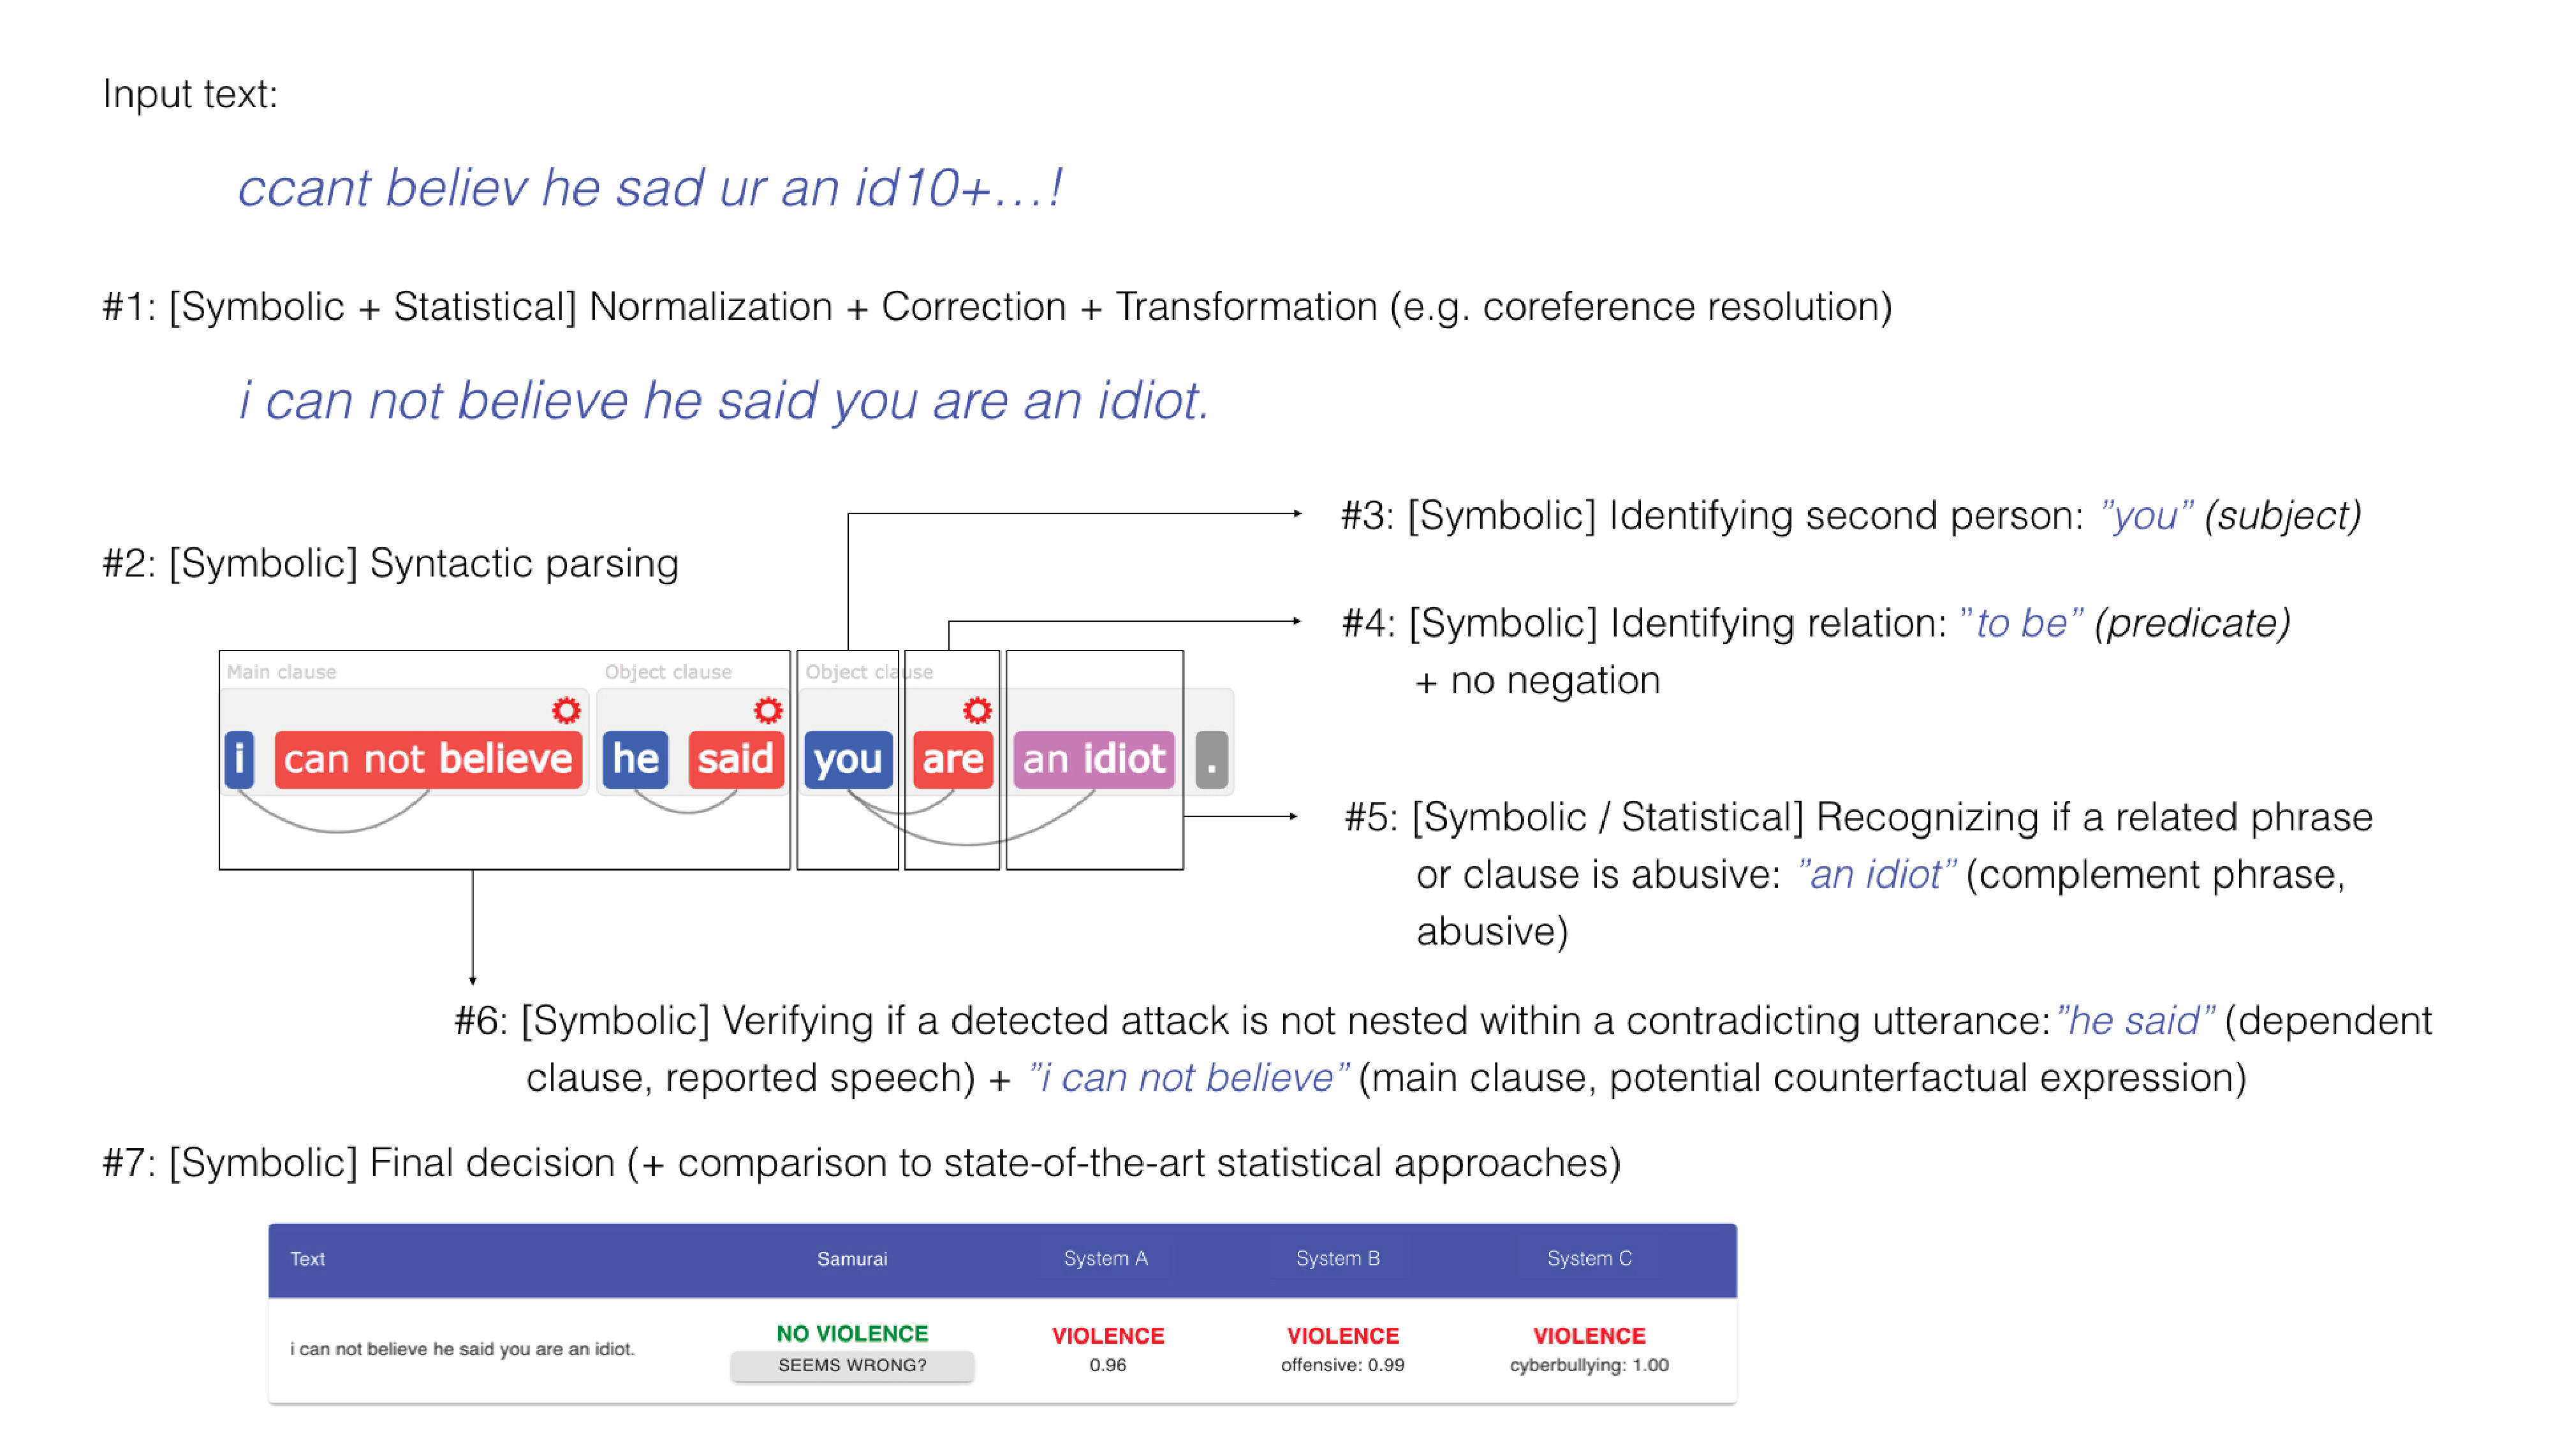
\includegraphics[width=\linewidth]{example.eps}
    \caption{Example of processing of one sentence by the applied Samurai technology.}
    \label{fig:samuraiexample}
\end{figure}

% In practice, this means that a whole variety of constructions can be
% detected without the need to construct a fixed list of dictionary words
% defined \textit{a priori}. Due to utilizing symbolic components that
% oversee statistical components, \{\textsf Samurai\} recognizes complex
% linguistic phenomena (such as indirect speech, rhetorical figures or
% counter-factual expressions) to distinguish personal attacks from normal
% communication, greatly reducing the number of false alarms as compared
% to others systems used for violence detection. An example of a comparison \todo{of what with what}
% can be seen in Figure \ref{fig:samuraiexample}, and a full benchmark was
% presented in (Ptaszyński et al., 2018).

% The detection models utilized in this research were designed to detect
% personal attacks targeted against a second person (e.g.~interlocutor,
% original author of a post) and a third person/group (e.g., other
% participants in the conversation, people not involved in the
% conversation, social groups, professional groups), except for public figures
% (e.g.~politicians, celebrities). With regards to the symbolic component of
% the system, by ``models'' we mean separate rules (such as, specifying a
% candidate for the presence of personal attack, such as the aggressive
% word ``idiot,'' which is further disambiguated with a syntactic rule of
% citation, e.g., ``{[}he\(\vert\)she\(\vert\)they{]} said {[}SUBJECT{]}
% {[}PREDICATE{]}'') or sets of rules, as seen in Figure
% \ref{fig:samuraiexample}, e.g.~normalization model contains rules for
% transcription normalization, citation detection model contains rules for
% citation, etc. With regards to the statistical component, by ``models''
% we refer to machine learning models trained on large data to classify an
% entry into one of the categories (e.g., true personal attack, or false
% positive) \todo{this doesn't make sense, Rafals comment}.

% Moreover, the symbolic component of the system uses two types of
% symbolic rules, namely ``narrow rules'' and ``wide rules.'' The former
% have smaller coverage (e.g., are triggered less often), but detect
% messages containing personal attacks with high
% a precision.\footnote{Precision is defined traditionally as the ratio of correctly detected instances among all detected instances.}
% The latter have wider coverage, but their precision is lower. We
% decided to set apart the ``narrow'' and ``wide'' subgroups of the
% detection models in order to increase the granularity of the analysis.
% Firstly, we took only the detection models designed to detect personal
% attacks targeted against second person. Secondly, we used these models
% on a dataset of 320,000 Reddit comments collected on 2019/05/06.
% Thirdly, we randomly picked at most hundred returned results for each
% low-level
% model\footnote{Low-level models are responsible for detecting low-level categories. Similarly, mid-level models detect mid-level categories, by combining several low-level models, etc.}
% (some models are triggered very often while others rarely, so using all
% instances would create too much bias). There were 390 low-level models
% but many of them returned less than 100 results. We verified them
% manually with the help of expert annotators trained in detection of
% personal attacks and selected only those models that achieved at least
% 90\% of precision. The models with fewer than 100 results were
% excluded from the selection. After this step, the ``narrow'' subgroup
% contained 43 out of 390 low-level models. Finally, we tested all of the
% ``narrow'' models on a large dataset of 477,851 Reddit comments
% collected between 2019/06/01 and 2019/08/31 from two subreddits
% (r/MensRights and r/TooAfraidToAsk). Each result of the ``narrow''
% models was verified manually by a trained annotator and the ``narrow''
% models collectively achieved the precision of 93.3\%. We also tested
% the rest of the ``wide'' models on random samples of 100 results for
% each model (from the previous dataset of 320,000 Reddit comments) and we
% excluded the models that achieved less than 80\% precision. The models
% with fewer than 100 results were not excluded from the ``wide'' group.
% In this simple setup we detected 24,251 texts containing ``wide''
% attacks, where:

% \begin{itemize}
% \item  5,717 (23.6\%) contained personal attacks against second person detected by the "narrow" models,
% \item  8,837 (36.4\%) contained personal attacks against second person detected by "wide" models
% % the models other than "narrow",
% \item  10,023 (41.3\%) contained personal attacks against third persons / groups.
% The sum exceeds 100\% because some of the comments contained personal attacks against both second person and third person / groups. For example, a comment ``Fu$\ast\ast$ you a$\ast\ast$hole, you know that girls from this school are real bit$\ast\ast$es" contains both types of personal attack.
% \end{itemize}
% \todo{table with recall precision tests - Rafals comment}














\section{Data analysis}\label{sec{analysis}}

\subsection{Data collection and exploration}\label{subsec:data-and-exploration}









We conducted a 6-months field experiment in a digital setting conducted on a popular Q\&A and news forum, Reddit (\url{www.reddit.com}). We formed treatment and control groups based on three main criteria:

\renewcommand{\labelenumii}{\Roman{enumii}}
 \begin{enumerate}
 \item During the intervention period, we have expected to have 20 active volunteers at any given time, each willing to conduct approximately 10 interventions a day.  So, we needed approximately 200 attacks daily generated by the treatment groups.
\item We first conducted a preliminary identification of users who regularly attack others to test interventions on them. The key issue here is that such users are not too common, and attacks are rather rare among other users. If instead we simply picked a random group of users with the intention of intervening in response to their online attacks, the sample size would have to be extremely large, and still the chance of observing enough attacks to draw any interesing conclusions from the reactions to our interventions would be low. Thus, we need to keep in mind that the group studied is not just users of Reddit, but rather users who for a least a few weeks tended to systematically attack others.

\item The identification of users who were active during the whole preliminary monitoring period was necessary to minimize the risk of attrition during the study. 
 \end{enumerate}

\noindent The user identification process was as follows:

\renewcommand{\labelenumii}{\Roman{enumii}}
 \begin{enumerate}
   \item First, we obtained 1 week of real-time umoderated data from Reddit (February 15-22. 2020), unmoderated data from Reddit. The content was downloaded from the data stream provided by pushshift.io. 
   \item Samurai Labs Artificial Intelligence for personal attacks detection was applied to identify those users who attacked others at least once within this period. This resulted in the identification of 93966 users. 
   \item We removed all accounts which we suspected not to be run by humans (AutoModerator and all users which had "bot" in the username string). This resulted in the removal of 388 users, thus 93578 were left on our list.
   \item Next, we removed those users who generated only 1 personal attack during the week. This step resulted in the removal of users generating the number of personal attacks below the third quartile (Q3). 20124 users were left in our group.
   \item We removed users who generated less than 14 comments during this week. It was not a lot, since 14 comments were below the 1st quartile (Q1: 28 comments), but such a criterion moved us in the direction of identification of those who are relatively active. This resulted in the removal of 2192 users, so 17932 were left.
   \item We discarded users whose personal attacks to all comments ratio was below 2\%. This means the inclusion in the sample of users above the 1st quartile of personal attacks to all comments ratio. 4422 users were removed, leaving us with a group of 13510.
   \item The next step of the process begun on  March 9, 2020, and lasted until May 5, 2020 (9 weeks). During this period we have monitored the activity of the identified group of 13510 users and applied further selection criteria to make sure we select those who were regularly active and attacked other users.
   \item The period of monitoring was divided into weeks. We have discarded those weeks during which technical difficulties occurred with \linebreak \url{pushshift.io} (resulting in missing data). So we have taken into consideration only 6 full weeks for the period.
   \item Users who generated at least 1 attack per week during 5 out of 6 weeks were identified. Initially, we planned to restrict the list to only those users who generate at least 1 attack during each week (6/6), but such a restrictive criterion led to only 255 users left, which was not enough for the study. The less restrictive criterion (at least 1 attack generated during 5/6 weeks) resulted in 694 people. 
   \item Next, we calculated the daily average number of personal attacks generated by the resulting group (357 attacks per day).
   \item Knowing that we need around 200 attacks per day  per treatment group (just enough for volunteers to keep up according to our assumption), we have randomly selected 195 users per each treatment group (normative and empathetic). The rest was delegated as a control group (304 users). 
   \item Some of those were further removed as t data visualisation  and content inspection helped to identify them as bots, or they ceased their activity during the period. We were left with the data on 440 users.

   
 \end{enumerate}


The duration of the experiment, 6 months, was divided into three 2-months periods. The first two months served as a monitoring period to properly select groups and establish baselines. The next 2 months served as a treatment period, during which groups received counter-speech comments from volunteers in response to personal attacks detected by the Artificial Intelligence-based system. The last 2-months served as the post-treatment monitoring period to gather the data needed to evaluate the effectiveness of interventions.
We started with an observation period on March 9, 2020, leading to  the intervention period starting on July 8, 2020,  following with  a further observation period starting on September 9, 2020,
and ending on November 20, 2020. The time series of attacks observed
and of interventions conducted can be inspected in Figure
\ref{fig:periodsPlot}, along with a quick search for weekly patterns.
Some of the users turned out to be bots, a few ceased to be active
during the experiment (with no strong reason to think this happened due
to them receiving an intervention) and a few received treatment of two
different types by accident (we relied on multiple volunteers and such
mistakes were likely to happen). Ultimately, in the time series data, we
ended up with data on 440 users.



\begin{figure}
\begin{center}\includegraphics[width=0.88\linewidth]{figures/periodsPlot-1} 

\includegraphics[width=0.88\linewidth]{figures/periodsPlot-2} \end{center}
\caption{Daily sums of attacks and interventions throughout the three experimental periods, with GAM smoothing (left) and daily attack sums from all  weeks in the experimental period plotted against week days (right)---no pattern seems to arise.}
\label{fig:periodsPlot}
\end{figure}


We analyzed the data from three perspectives: we used the daily data to
(1) build seven time series models estimating the impact of individual
interventions at lags 1-7 days, and (2) to study the impact of the
cumulative number of  interventions received as the experiment
progressed, and (3) we used aggregated data to run a long term
before-and after analysis, comparing the summarized aggression levels
before and after the intervention period.



Before we move to the analysis, let us inspect the data. First, at the
aggregated level, the data involve the variables listed in Table
\ref{tab:baaVars}.\footnote{Further variables were defined in terms of those, in particular, we will be predicting \textsf{AdiffS} which is the standardized difference  \textsf{AA}-\textsf{AB}, and \textsf{AdiffS}, which is the standardized difference \textsf{CA}-\textsf{CB}.The  standardized variables are systematically named  $\langle$variable\char`_name$\rangle$S.} The distribution of \textsf{IC} in the treatment groups is visualized in
Figure \ref{fig:interventionsDistro}. Note that the distributions are
somewhat different, even though the total intervention counts are
similar. The issue is discussed in Section XXXXX.\todo{add ref}


\vspace{1mm}
\footnotesize

\normalsize

\begin{table}
\centering
\begin{tabular}{ll}
\toprule
variable  explanation\\
\midrule
\cellcolor{gray!6}{AB}  \cellcolor{gray!6}{attacks before (pre-treatment)}\\
AD  attacks during (the treatment period)\\
\cellcolor{gray!6}{AA}  \cellcolor{gray!6}{attacks after (post-treatment)}\\
CB  comments before\\
\cellcolor{gray!6}{CD}  \cellcolor{gray!6}{comments during}\\
CA  comments after\\
\cellcolor{gray!6}{group}  \cellcolor{gray!6}{treatment group}\\
IC  intervention count\\
\bottomrule
\end{tabular}

\caption{Variables involved in the before-and-after analysis.}
\label{tab:baaVars}
\end{table}



\begin{figure}

\begin{center}\includegraphics[width=.88\linewidth]{figures/interventionsDistroPlot-1} \end{center}
\caption{Distribution of daily interventions (by treatment group).}
\label{fig:interventionsDistro}
\end{figure}

Second, in the distribution of standardized difference in attacks, the
peaks of distributions are shifted a bit between the groups, with lowest
median for the normative group, but the differences seem minor (Figure
\ref{fig:violJoint}). This might suggest no impact of the interventions.
This conclusion would be too hasty, as the impact of other predictor
variables and interactions involved can mask actual associations.




\begin{figure}

\begin{center}\includegraphics[width=1\linewidth]{figures/violJoint-1} \end{center}
\caption{Empirical distribution of change in attacks (by treatment group).}
\label{fig:violJoint}
\end{figure}

To see how this masking can occur, let us inspect changes in attacks
against intervention counts. It turns out that restricting attention to
various aggression levels in the before period results in fairly strong
changes to the regression lines (Figure \ref{fig:linearShift}). This
suggests we should keep an eye out for interactions with aggression
before in the analysis, and that the initial comparison of means or
medians between groups might be misleading if the effects in different
volume groups are different and to some extent cancel each other.



\begin{figure}

\begin{center}\includegraphics[width=1\linewidth]{figures/fig:linearShift-1} \end{center}
\caption{Change in attacks vs the number of interventions received by treatment group, jittered with  linear smoothing.}
\label{fig:linearShift}
\end{figure}

\normalsize

Further insights, undermining the initial impression suggested by Figure
\ref{fig:violJoint}, can be obtained by visualizing individual time
series. Figure \ref{fig:tsVis} contains six fairly typical examples.






\begin{figure}

\begin{center}\includegraphics[width=1\linewidth]{figures/fig:tsVisPlot6-1} \end{center}
\caption{Examples of individual time series. Black points are attacks (smoothed in blue), red lines represent the cumulative number of interventions received (lag 3) divided by 10, gray lines represent overall activity level divided by a variable divider listed in the subtitle. Divisions introduced for visual comparability of general trends.}
\label{fig:tsVis}
\end{figure}

\normalsize

The general phenomenon is that while in the control group attacks tend
not to diminish, unless activity itself diminishes, they tend to
diminish in the normative group (although the more aggressive the user
is, the less of an impact can be observed), and in the empathetic group
if the user is not very aggressive. Of course, visualization of
individual cases (which the reader might suspect to be cherry-picked) is
no replacement for statistical analysis, to which we will now move.



\subsection{Causal thinking, choice of variables and
models}\label{subsec:causal-thinking-choice-of-variables-and-models}

First, we inspect correlations between predictors to avoid multicolinearity, as highly correlated predictors do not improve predictive performance and artificially inflate uncertainty in their corresponding coefficients in the models. We then develop
a plausible causal model of the situation (Figure
\ref{fig:correlations}). It turns out that to avoid multicolinearity we
cannot condition on CDS (comments during, standardized) if we condition on CAS (comments after, standardized) or CBS (comments before, standardized). Similarly, for
the time series data, since activity levels in particular day slices are
correlated, it will not be useful to condition on more than one
auto-regressive element (and since the predictive power is the highest
for lag 1 with no discoverable weekly patterns, we will not go further
than lag 1).

To choose the right variables to condition (or not condition) on to
identify the causal effect of the interventions, we need to think about
the causal structure of the problem. Comments during (the intervention period) impact attacks
during, which trigger interventions. Unmeasured user features cause
comments before (the intervention period), which impact attacks before directly. Comments during
(their impact on ADS is already included) impact attacks during directly
and comments after, which impact attacks after
directly. Intervention count impacts attacks after and comments after.
The same directions of impact are included for intervention type.
Finally, comments through time are connected causally, and so are
attacks. The structure for the time series data is analogous, except now
instead of before and after, we have multiple daily indices.



\begin{figure}

\begin{center}\includegraphics[width=0.48\linewidth]{figures/correlations-1} \includegraphics[width=0.48\linewidth]{figures/correlations-2} \end{center}

\caption{Correlations between predictors (left) and a plausible causal model (right) used in the before-and-after analysis.}
\label{fig:correlations}
\end{figure}



What do we learn from causal considerations? \textsf{IT} has no backdoor
paths, but \textsf{IC} does, so we need to make sure these are closed to
avoid including spurious correlations in our analysis. There are in fact
65 different paths from \textsf{IC} to \textsf{AAC}. Crucially, all
backdoor paths go through \textsf{ADS}, which then becomes either a fork
or a pipe, so all backdoor paths can be closed by conditioning on
\textsf{ADS}. Moreover there is only one directed indirect path, it goes
through \textsf{CAS}, so we should not condition on \textsf{CAS} if we
are to identify total causal effect of \textsf{IC} on attacks, including
the impact mediated by its impact on comments. We might be interested in
the direct effect of \textsf{IC} and \textsf{IT} on \textsf{AAS}, but
then we also need to block indirect causal paths from the intervention
to the outcome. For such an evaluation we would need to also condition
on \textsf{CAS} and block all backdoor paths from \textsf{CAS} to
\textsf{AAS}. This, however, given the causal model, cannot be achieved,
as it would required conditioning on unobserved user features. That is,
we do not think direct causal effect is identifiable.

Analogous considerations apply to the time series model for the total
impact of individual interventions received exactly \(k\) days before
(in our case, \(k\in \{1, \dots, 7\}\)). The situation, however, is
somewhat different for the impact of the total number of cumulative
interventions received so far. The trouble is, for example, that if a
user received so far a number of interventions until yesterday, some of
them had been received before yesterday and those had already impacted
their aggression level yesterday. In other words, conditioning on lagged
attacks leads to the post-treatment bias and should be
avoided.\footnote{In fact, in the aggregated data analysis, we will be predicting the standardized difference between attacks before and after (\textsf{ADiffS}), and the standardized difference between comments, before and after (\textsf{CDiffS}), but the general points about the nodes involved apply also to defined nodes.  As already discussed, we do not include \textsf{CDS} because of its strong correlation with \textsf{CBS}. We also do not condition on \textsf{ABS} when modeling \textsf{ADiffS} (or on \textsf{CBS} when modeling \textsf{CDiffS})---not only because it has a pretty strong correlation with another predictor (\textsf{ADS}), but rather also because it is used to define the output variable. In such a set-up, it is clear that a model including \textsf{ABS} would have better predictive power, but since a definitional connection is present, thinking that its inclusion in the model tells us something about causality  would be misled.}

Otherwise, it's open season for the other variables and interactions
between them, and our decision to include or exclude them in the model
will be guided by information-theoretic criterion of predictive power, whose more detailed explanation is  included in the appendix, the so-called
Widely Acceptable Information Criterion:
\[
\mathsf{WAIC(y, \Theta)}  = -2 (\mathsf{lppd} - \overbrace{\sum_i var_\theta \mathsf{log} p (y_i \vert \theta)}^{\mathsf{penalty}})
\]
We also use  posterior predictive checks in cases in which the likelihood
functions used by the models to be compared are different and
information-theoretic calculations might be misleading. In such cases we
investigated the ratio of actual observations included in the 50\% and
in the 89\% posterior predictive distribution, and the models for which
higher ratios were observed in both were selected (no case of diverging
evaluation for the two criteria has been observed).

In our model building we used the \textsf{rethinking} package,
except for the cumulative impact time series models, where it becomes
computationally unfeasible, in which case we built models in
\textsf{Rstan} directly. Moreover, for the time series analysis we will
build hierarchical Bayesian models which tend to have around
\(u \times 2p + 2p\) parameters (we will explain later why), which means
that for 440 users our final model with interaction with six predictors
would have \(440 \times 12 + 12 = 5292\) parameters, and 
have to be trained on daily data for 7 variables collected for six months. The
building of such a model on a modern computer takes days. Since in
reaching this model we needed to build multiple somewhat simpler models
or models with different structures and test their performance, model
selection on the full data set was unfeasible. That is, in the time
series analysis in model selection at each step we compared models
(sometimes built with quadratic approximation) with respect to three
independent samples for \(40, 60\) and \(60\) users. We made the
decision only if a given model structure performed better on all these
subsets (which was usually the case, so the model selection criteria
gave us pretty robust answers). For the most complicated model of the
impact of cumulative number of interventions, building a single model
for the whole data set was not computationally feasible (computation
time does not increase linearly with the number of users included in the
dataset), so we randomly split the dataset 
and provided results for the subgrous---the results were not very divergent and the highest posterior density intervals were not very wide.





For the time series, the model that the procedure led us to is as follows (see the appendix for a detailed explanation of how this model has been reached):

\footnotesize

\begin{center}
\begin{tabular}{c}
$\mathsf{attacks}_i  \sim  \mathsf{NegativeBinomial}(\lambda_i, \phi_{\mathsf{userID[i]}} ) $\\
$log(\lambda_i)  =  l_{\mathsf{userID[i]}} +
                  a_{\mathsf{userID[i]}} \times \mathsf{attacksL1} +
                  c_{\mathsf{userID[i]}} \times \mathsf{act} + $\\
$                   + 
       i1control_{\mathsf{userID[i]}} \times  \mathsf{control} \times \mathsf{intL1D}  +$ \\$         +  i1emp_{\mathsf{userID[i]}} \times  \mathsf{emp} \times \mathsf{intL1D}  +$ \\$
              +  i1norm_{\mathsf{userID[i]}} \times  \mathsf{norm} \times \mathsf{intL1D}
                          $\\ 
$  l_{\mathsf{userID[i]}}   \sim \textsf{Norm}(\bar{l}, \bar{\sigma_l}) $\\
$  a_{\mathsf{userID[i]}}  \sim \textsf{Norm}(\bar{a}, \bar{\sigma_a}) $\\
$  c_{\mathsf{userID[i]}}  \sim \textsf{Norm}(\bar{c}, \bar{\sigma_c}) $\\
 $ i1control_{\mathsf{userID[i]}}  \sim  \textsf{Norm}(i1controlOverall,\bar{\sigma_{i1}})$ \\
$   i1emp_{\mathsf{userID[i]}}  \sim  \textsf{Norm}(i1empOverall, \bar{\sigma_{i1}})$\\  
 $ i1norm_{\mathsf{userID[i]}}   \sim  
     \textsf{Norm}(i1normOverall, \bar{\sigma_{i1}})$\\
$     i1controlOverall  \sim  \textsf{Norm}(0,.2)$\\
$    i1empOverall   \sim  \textsf{Norm}(0,.2) $\\
$    i1normOverall   \sim  \textsf{Norm}(0,.2) $\\
$    \bar{\lambda}   \sim  \textsf{Norm}(.00001, 2.5) $\\
$    \bar{\sigma_l}  \sim  \mathsf{Exp}(1.5)$\\
$    \bar{a}  \sim \textsf{Norm}(0, .2) $\\
$    \bar{\sigma_a}  \sim  \mathsf{Exp}(5) $\\
$    \bar{c}  \sim  \mathsf{Norm}(0, .2)$\\
$    \bar{\sigma_c}  \sim \mathsf{Exp}(5) $\\
$    \bar{\sigma_{i1}}  \sim  \mathsf{Exp}(5)
$
\end{tabular}
\end{center}

\normalsize



\noindent This might seem somewhat confusing, so let us disentangle this maze:

\begin{itemize}
\item Each user has their own baseline aggression level, $l_{\mathsf{userID[i]}}$. \item However, these individual aggression levels are not disconnected, they come from a distribution themselves, $\textsf{Norm}(\bar{l}, \bar{\sigma_l})$. $\bar{l}$ is the mean baseline aggression level for the whole population, and $\bar{\sigma_l}$ is the standard deviation of this distribution. These general parameters are to be estimated along with the individual ones.
\item Then  there are individual auto regression coefficients     $a_{\mathsf{userID[i]}}$, which capture the correlation between  yesterday's attacks with today's attacks, so to speak. These also come from a general distribution \linebreak  $\textsf{Norm}(\bar{a}, \bar{\sigma_a})$, with its own general parameters to be estimated.
\item Next, there are individual user's coefficients connecting the user's activity on a given day with their aggression on the same day,  $c_{\mathsf{userID[i]}}$, all coming from a general distribution $\textsf{Norm}(\bar{c}, \bar{\sigma_c})$ whose parameters are also to be estimated.
\item For any particular treatment group, say, empathy, we have a user level coefficient $i1emp_{\mathsf{userID[i]}}$, which is activated if the user is in the empathy group (that is, we multiply by the indicator variable $\mathsf{emp}$) and then applied to the number of interventions received the day before (lag 1). Similarly for the two other groups. These user-level parameters come from the distribution $\textsf{Norm}(i1empOverall, \bar{\sigma_{i1}})$, whose parameters are to be estimated.
\item Finally, prior predictive check was used to choose priors for the general coefficients. 
\end{itemize}




For the impact of the cumulative number of interventions (we will only
use lag 3 for reasons that will become clear), since the range of values
of the predictor is wider, for computational feasibility we further
needed to restrict coefficients to lie between -3 and 2, but these
values are not plausible values of the parameters anyway
(\(exp(-3) \approx 0.04\) and \(exp(2) \approx 7.38\)). The model for
the cumulative impact was tested with and without interaction with
overall aggression in the before period, without the use of attacks on a
given day (as already explained, to avoid the post-treatment bias). The
two relevant options   are:



\footnotesize


\begin{center}
\begin{tabular}{c}
$log(\lambda_i)  =  l_{\mathsf{userID[i]}}  + c_{\mathsf{userID[i]}} \times \mathsf{act} + 
      ic3control_{\mathsf{userID[i]}} \times  \mathsf{control} \times \mathsf{intCL3D}  + $\\$  + 
            ic3emp_{\mathsf{userID[i]}} \times  \mathsf{emp} \times \mathsf{intCL3D}  + $\\  
    $  ic3norm_{\mathsf{userID[i]}} \times  \mathsf{norm} \times \mathsf{intCL3D}$\\
$log(\lambda_i)  =  l_{\mathsf{userID[i]}}  + c_{\mathsf{userID[i]}} \times  act + $\\$  + 
      ic3control_{\mathsf{userID[i]}} \times   \mathsf{control} \times  \mathsf{intCL3D}  + $\\$  + icabst3control_{\mathsf{userID[i]}} \times   \mathsf{control} \times  \mathsf{intCL3D} \times  \mathsf{abst} + $\\ 
        \end{tabular}
\end{center}

\begin{center}
\begin{tabular}{c}
  $log(\lambda_i)  =  l_{\mathsf{userID[i]}}  + c_{\mathsf{userID[i]}} \times \mathsf{act} + 
      ic3control_{\mathsf{userID[i]}} \times  \mathsf{control} \times \mathsf{intCL3D}  + $\\ $ +    ic3emp_{\mathsf{userID[i]}} \times   \mathsf{emp} \times  \mathsf{intCL3D}  + $\\$  + icabst3emp_{\mathsf{userID[i]}} \times   \mathsf{emp} \times  \mathsf{intCL3D}  \times  \mathsf{abst} + $\\ $ +
        ic3norm_{\mathsf{userID[i]}}] \times   \mathsf{norm} \times  \mathsf{intCL3D} + $\\ $ + icabst3norm_{\mathsf{userID[i]}} \times   \mathsf{norm} \times  \mathsf{intCL3D} \times  \mathsf{abst} 
        $
        \end{tabular}
\end{center}


\normalsize

The models employing the second formula were superior in performance. It
is not surprising that once attacks on a given day were removed from
predictor, the overall aggression levels in the before period became
predictive. The price to pay, however, is that now to obtain a
user-specific multiplicative interpretation of the impact of cumulative
interventions, we need to put the two elements together while
multiplying one by the user's overall aggression and only then
exponentiate, that is we need to inspect, for instance,
\(exp(ic3emp_{\mathsf{userID[i]}} + icabst3emp_{\mathsf{userID[i]}} \times \mathsf{abst}[i])\),
instead of simply looking at \(exp(ic3emp_{\mathsf{userID[i]}})\).






Finally, in the before-and-after analysis, we put aside the time series
element, and look at aggregated counts before and after the treatment
period, thus obtaining a more of a long-term effect analysis. Moreover,
this time we standardize counts, obtaining continuous variables and
employing normal distribution in the likelihoods, thus also making sure
the overall results are robust under a spectrum of modeling choices. We
build and compared multiple additive models where the outcome variable
is normally distributed around the predicted mean, which is a linear
function of predictors (possibly with interactions). Our general criteria
led to the model whose specification is as follows (we also selected
regularizing prior parameters using prior predictive checks to avoid
unreasonably narrow overall prior distributions, see the appendix for a longer explanation):


\footnotesize


\begin{center}
\begin{tabular}{c}
$\mathsf{AdiffS}  \sim \textsf{Norm}(\mu, \sigma)$\\
$\mu_i  = \alpha + \beta_{\mathsf{ADS}}[\mathsf{group}_i]\times \mathsf{ADS} + \beta_{\mathsf{group}_i}  +
 \beta_{\mathsf{IC}}[\mathsf{group}_i]\times \mathsf{IC} + $\\
$  + \beta_{\mathsf{ADSIC}}\times \mathsf{ADS} \times \mathsf{IC} + \beta_{\mathsf{CBS}}[\mathsf{group}_i] \times \mathsf{CBS}$\\
$ \alpha  \sim \textsf{Norm}(0,.3)$\\
$\beta_{\mathsf{ADS}}[\mathsf{group}_i]  \sim \textsf{Norm}(0,.3)$\\
$\beta_{\mathsf{group}_i}  \sim \textsf{Norm}(0,.3)$\\
$\beta_{\mathsf{IC}}[\mathsf{group}_i]  \sim \textsf{Norm}(0,.3)$\\
$ \beta_{\mathsf{ADSIC}}  \sim \textsf{Norm}(0,.3)$\\
$ \beta_{\mathsf{CBS}}[\mathsf{group}_i] \sim \textsf{Norm}(0,.3)$\\
\end{tabular}
\end{center}

\normalsize 

That is, we take the resulting mean to be the result of the general
average (\(\alpha\)) and the impact of the following coefficients:
group-specific coefficient for \textsf{ADS}, group coefficient,
group-specific coefficient for \textsf{IC}, interaction coefficient for
\textsf{ADS} and \textsf{IC}, and group-specific coefficient for
\textsf{CBS}. This is plausible \emph{prima facie}, as which group a
user belongs to might have an impact on how the number of attacks during
the treatment is related to the number of attacks after, the role of
the intervention count, and the role of comments before. Moreover, the
levels of aggressive behavior displayed by the user during treatment
might have an impact on the role played by the intervention count.









\subsection{Results}\label{subsec:resultss}


\subsubsection{Interventions on a given
day}\label{subsubsec:interventions-on-a-given-day}




We built seven separate models for the impact of interventions \(k\)
days ago, \(1\leq k \leq 7\). In Figure \ref{fig:dailyResults} we
visualize the results for the three groups, with jitter based on user
aggression in the before period.


\begin{sidewaysfigure}

\begin{center}\includegraphics[width=1\linewidth]{ figures/fig:dailyResultsPlot-1} \end{center}
\caption{Impact of interventions received lag $1\leq k \leq 7$ on attacks on a given day. High-level coefficients are pictured in black.}
\label{fig:dailyResults}
\end{sidewaysfigure}

Notice that in short term, interventions actually increase aggression
the next day (even taking the user's yesterday's aggression and today's
activity in consideration). The effect, however, quickly wears off.


\subsubsection{Cumulative sum of
interventions}\label{subsubsec:cumulative-sum-of-interventions}




In our analysis of the effect of the cumulative number of interventions
received so far, however, we intend separate this short-term effect from
the long-term effect. To achieve this, we lag the cumulative
interventions variable by 3, so that we're giving the user the minimal
number of days needed for the short-term effect to wane. The individual
users' multiplicative impact coefficients are visualized in Figure
\ref{fig:cumulativeResultsPlot}.


\begin{figure}

\begin{center}\includegraphics[width=.8\linewidth]{ figures/fig:cumulativeResultsPlot-1} \includegraphics[width=.8\linewidth]{ figures/fig:cumulativeResultsPlot-2} \end{center}
\caption{Multiplicative impact of cumulative interventions lag 3 on attacks. Individual users' coefficents only, full range (top), and with attention restricted to the bulk of the sample. Sub-sample coefficients depend on aggression and are represented as lines, colored by sub-sample. Note low number and high uncertainty for highly aggressive users, which motivate the restriction of the $x$ axis for inspection.}
\label{fig:cumulativeResultsPlot}
\end{figure}

\normalsize

The efficiency of normative interventions seems overall higher, except
for low-aggression users, for which empathetic interventions might be
equally or more useful. Importantly, linear extrapolation to extreme
values might be misleading, so let us inspect on what happens with the
general level multiplicative coefficients at the levels of aggression
which are actually quite common, that is, at the 1st, 2nd and 3rd
quartile (with respect to \(\mathsf{abst}\)). This indicates that for
the bulk of the sample the impact of cumulative interventions has been
negative, slightly more so on users with lower aggression levels.






\begin{figure}

\begin{center}\includegraphics[width=1\linewidth]{ figures/fig:cumulativeResultsGeenralPlot-1} \end{center}
\caption{Multiplicative impact of cumulative interventions lag 3 on attacks. General level coefficents only, in three quantiles (.25, .5, .75). Colored by sub-sample.}
\label{fig:cumulativeResultsGeneralPlot}
\end{figure}


\subsubsection{Long term before/after
analysis}\label{subsubsec:long-term-beforeafter-analysis}

The general problem with interpreting  models of this complexity involving
interaction is  that coefficients are not directly interpretable. For this reason, it is better
to plot predicted effects for various combinations of predictors. In the
construction of the plots we rely on the following:

\begin{itemize}
\item The values \textsf{ADS} range from -.67 to 10, with approximately 30\% below -.5, around 80\% below .3, and around 95\% below 1.7, so we use these three settings of this variable in our visualizations. 

\item The values \textsf{CBS} range from -.82 to 18.3, with approximately 30\% below -.4, around 80\% below .3, and around 95\% below 1.3, so we use these three settings of this variable in our visualizations. 


\end{itemize}

% \begin{figure}
% \begin{center}\includegraphics[width=1\linewidth]{ figures/unnamed-chunk-3-1} \end{center}
% \caption{The final model coefficients.}
% \label{fig:coeffs}
% \end{figure}




Grouped before-and-after predicted change of attacks by the levels we
just listed are visualized in Figure \ref{fig:predictedChange}. For more clarity, let's inspect predicted contrasts, here understood as
distances from the control group mean, by activity level, first versus
CBS (comments before, standardized, Figure \ref{fig:ContrastCBS}), then
versus ADS (attacks during, standardized, Figure \ref{fig:ContrastADS}).


\begin{figure}

\begin{center}\includegraphics[width=1\linewidth]{ figures/unnamed-chunk-5-1} \end{center}
\caption{Predicted change in attacks, depending on user’s activity level
(CBS: comments before, standardized) and how aggressive overall they
were (ADS: attacks during, standardized). The more aggressive and active
the users, the higher the attacks drop in the normative group, slight drop
correlated with emotive interventions for not too active users.}
\label{fig:predictedChange}
\end{figure}







\begin{figure}

\begin{center}\includegraphics[width=1\linewidth]{ figures/unnamed-chunk-7-1} \end{center}
\caption{Predicted contrasts (difference in attacks as compared to the control group)
for the two treatment groups vs activity before the treatment. Notice that
empathetic interventions correlated with decreased attacks for less active
users, but performed worse than normative interventions for more active
users. Normative interventions, in contrast, seem to have better impact on
 more active users.}
\label{fig:ContrastCBS}
\end{figure}




\begin{figure}

\begin{center}\includegraphics[width=1\linewidth]{ figures/unnamed-chunk-9-1} \end{center}
\caption{Predicted contrasts (difference in attacks as compared to the control group)
for the two treatment groups vs aggression during the treatment period.
Notice that empathetic interventions correlated with decreased attacks for
less aggressive users, but performed worse than normative interventions for
more aggressive users. Normative interventions, in contrast, seem to have
better impact on  more aggressive users.}
\label{fig:ContrastADS}
\end{figure}




Now, let's inspect the impact of intervention counts by treatment type
by looking at contrasts (distances from the control group mean) with
89\% HPDIs by IC (intervention count). Notice the predicted effect of IC
is weaker than group membership, so for visibility the \(y\)-axis has a
smaller range. Also, not enough data was available to reliably estimate
uncertainty for IC above 20, hence the restriction on the \(x\)-axis
(already at lower values, lack of estimates is visible for the more
extreme settings).





\begin{figure}

\begin{center}\includegraphics[width=1\linewidth]{ figures/visICPlot-1} \end{center}
\caption{Contrasts (change in attacks as compared to the control group) vs the number
of interventions received. Note that repeating empathetic interventions
correlates with decreased attacks, while repeating normative interventions
is counterproductive.}
\label{fig:ContrastsIC}
\end{figure}



\section{Discussion}














\section{Volunteer engagement and impact of competitions}


\subsection{The challenge of keeping volunteers engaged}


\subsection{Volunteer activity  data analysis}


The winning model, given our model selection method, is specified as
follows:


\footnotesize


\begin{center}
\begin{tabular}{c}
$\mathsf{interventions} \sim \mathsf{NegativeBinomial} (\lambda,\phi) $\\
$log(\lambda) = l_\mathsf{volunteerID[i]} + enth_\mathsf{ volunteerID[i]} \times \mathsf{daysOfProject} + comp_\mathsf{volunteerID[i]} \times \mathsf{competition}$\\  
$l_\mathsf{ volunteerID[i] }  \sim \mathsf{Norm}(lbar,lsigmabar) $\\
$lbar \sim \mathsf{Norm}(2, .9)$\\
$lsigmabar, enthsigmabar, compsigmabar \sim  \mathsf{Exp}(.5) $\\
$enth _\mathsf{ volunteerID[i] }  \sim \mathsf{Norm}(enthbar, enthsigmabar)$\\
$comp_\mathsf{ volunteerID[i] } \sim \mathsf{Norm}(compbar, compsigmabar) $\\
$enthbar, compbar \sim  \mathsf{Norm}(0, .3)$\\
$ \phi =  puser_\mathsf{ volunteerID[i] } $ \\
$ puser_\mathsf{ volunteerID[i] } \sim \mathsf{Exp}(1)$
\end{tabular}
\end{center}


\normalsize


Intuitively, volunteer interventions are assumed to have negative
binomial distribution around their own expected value \(\lambda\) and
individualized dispersion parameters \(\phi\). On each day each a user
has their own daily expected value, which is determined by the following
factors:

\begin{itemize}
\item First, there's user's individual baseline activity for the whole treatment period, $l_\mathsf{ volunteerID[i] }$.
\item next, each user has their own dispersion parameter,  $puser_\mathsf{ volunteerID[i] }$.
\item then, there is (usually dwindling) enthusiasm: the impact of time on that user, $enth_\mathsf{volunteerID[i]} $ to be (after exponentiation) multiplied by the number of days that have passed since the experiment started,
\item finally, we have the impact that the presence of competitions made on a user, $comp_\mathsf{ volunteerID[i] }$, which (after exponentiation) becomes the activity multiplier to be applied during competitions only.
\end{itemize}

\noindent Moreover, the model is hierarchical: the individual level
parameters are drawn from distributions whose parameters are in turn to
be estimated as well. Thus, \(lbar\) is the overall baseline for the
whole group, \(enthbar\) is the overall estimated group enthusiasm
coefficient, and \(compbar\) is the overall estimated competition impact
coefficient (all of them come with their own nuisance sigma parameters).

\noindent All of these parameters are given priors in a manner analogous
to the introduction of priors for the other time series models, as
explained in the appendix.\footnote{Interestingly, if we are interested
  in the causal effect of competitions, we should not use an
  auto-regressive predictor. If we auto-regress on a lag in the
  \([1,7]\) range, for some days we will be conditioning on
  interventions conducted during the same competition, which will
  already contain some information about the impact of that competition.
  In other words, auto-regression with short lags would lead to
  post-treatment bias. On the other hand, auto-regression with longer
  lags would either lead to dropping a lot of data in the beginning
  (where lagged information is not available), or degenerate the
  analysis by using 0s for missing lagged values in a long initial
  period. All this without much gain, as we have already inspected null
  models with auto-regression with large lags and they do not lead to
  performance improvement.}

Raw data and daily means are illustrated in Figure
\ref{fig:volunteersBasic}, and the individualized totals with the key
coefficients based on the trained model are illustrated in Figure
\ref{fig:volunteersModel}.

\begin{figure}

\begin{center}\includegraphics[width=1\linewidth]{figures/fig:volunteersBasic5-1} \end{center}
\caption{Daily individual voilunteer intervention counts accross time with competition periods marked (top) and daily group intervention means grouped by whether a competition was ongoing (bottom). Note most of high means in the non-competition period are in the first week.}
\label{fig:volunteersBasic}
\end{figure}

\begin{figure}

\begin{center}\includegraphics[width=1\linewidth,angle=90]{figures/fig:volunteersModel17-1} \end{center}
\caption{Volunteer total engagement with their daily baseline and multipliers for enthusiasm and impact of competition. Pointranges represent individual level coefficients, group coefficients are represented by black lines with shaded 89\% HPDI areas.}
\label{fig:volunteersModel}
\end{figure}
















%% The Appendices part is started with the command \appendix;
%% appendix sections are then done as normal sections
\appendix


\section{Explanation of WAIC}

 Let  $y$ be the observations and $\Theta$  a posterior distribution.
First, log-pointwise-predictive-density is defined by:
\[
\mathsf{lppd}(y, \Theta)  = \sum_i log\frac{1}{S}\sum_s p (y_i\vert \Theta_s)
\]
\noindent where $S$ is the number of samples in the posterior, and $\Theta_s$ 
is the $s$-th combination of sampled parameter values in the posterior distribution. That is, 
for each observation and each combination of 
parameters in the posterior we first compute its density, then 
we take the average density of that observation over all combinations of parameters in the posterior,
and  then take the logarithm. Finally, we sum these values up for all the observations. Crucially, when comparing posterior distributions with respect to the same dataset, \textsf{lppd}s are proportional
 to unbiased estimates of their divergence from the real distribution (note that it is \emph{only} 
 proportional, and for this reason can be used for comparison of distributions 
 only and makes no intuitive sense on its own).  However, \textsf{lppd} always improves
  as the model gets more complex, so for model comparison it makes more sense to use 
 the Widely Applicable Information Criterion (WAIC), which is an approximation of the out-of-sample deviance that converges to the cross-validation approximation in a large sample. It  is defined as
 the log-posterior-predictive-density with an additional
  penalty proportional to the variance in the
  posterior predictions:
\[
\mathsf{WAIC(y, \Theta)} = -2 (\mathsf{lppd} - \overbrace{\sum_i var_\theta \mathsf{log} p (y_i \vert \theta)}^{\mathsf{penalty}})
 \]
\noindent  Thus to construct the penalty, we calculate the variance in log-probabilities for each observation and sum them up. Because of the analogy to Akaike's criterion, the penalty is sometimes called the effective number of parameters, $p_{\mathsf{WAIC}}$. 
How does WAIC compare to other information criteria?  AIC uses MAP estimates instead of the posterior and requires that priors be flat or overwhelmed by the likelihood, and assumes that the posterior distribution is approximately multivariate Gaussian and the sample size is  much greater  than the number of parameters used in the model. Bayesian Information Criterion (BIC) also requires flat priors and uses MAP estimates. WAIC does not make these assumptions, and provides almost exactly the same results as AIC, when AIC’s assumptions are met.


\section{Time series model
selection}\label{sec:time-series-model-selection}

Suppose we are interested in the impact of interventions received \(n\)
days ago. We started with a simple null model that uses the Poisson
distribution, with either uses a single \(\lambda\) for all the users,
or user-specific \(\lambda\)s. The first Bayesian model has the
following structure: 


\footnotesize


\begin{center}
\begin{tabular}{c}
$\mathsf{attacks_i}  \sim  \textsf{Poisson}( \lambda)$\\$
    log(\lambda)   =  l $\\$
    l  \sim  \textsf{Norm}(.05,2.8)$
\end{tabular}
\end{center}

\normalsize

and the user-specific coefficient model had the following structure:


\footnotesize


\begin{center}
\begin{tabular}{c}
$\mathsf{attacks}_i  \sim  \textsf{Poisson}( \lambda_i)$\\$ 
    log(\lambda_i)   =  l_{\mathsf{userID[i]}} $\\$
    l_{\mathsf{userID[i]}}  \sim  \textsf{Norm}(.05,2.8)$
\end{tabular}
\end{center}


\normalsize

The priors were chosen using prior predictive check, so that the 89\%
density intervals reached between 0 and 34, with median around 1. Given
our prior experience with similar user datasets this is a fairly wide
informative prior. The comparison, unsurprisingly, preferred the
user-specific \(\lambda\)s.

Next, we introduced the auto-regressive element, conditioning on
yesterday's attacks. The choice of priors for the auto-regression
coefficient is guided by the visualization (intuitive direct
understanding of the values is made difficult by the fact that the
predictors work on the logarithmic scale) and the fact that larger
values would result in a unreasonably extreme impact of yesterday's
attacks. 



\footnotesize

\begin{center}
\begin{tabular}{c}
$\mathsf{attacks}_i  \sim  \textsf{Poisson}( \lambda_i)$\\$ 
    log(\lambda_i)   =  l_{\mathsf{userID[i]}} + a_{\mathsf{userID[i]}} \times \mathsf{attacksL1}$\\$
    l_{\mathsf{userID[i]}}  \sim  \textsf{Norm}(.05,2.8)$\\$
    a_{\mathsf{userID[i]}}  \sim \textsf{Norm}(0,.2)$
\end{tabular}
\end{center}


\normalsize

Next, we added today's activity level as a predictor, with user-specific
coefficients. Adding activity levels helps. Note also that our priors
taken separately were made more narrow, to preserve the overall width of
the prior predictive distribution (this will be the usual strategy as we
progress). 


\footnotesize


\begin{center}
\begin{tabular}{c}
$\mathsf{attacks}_i   \sim  \textsf{Poisson}( \lambda_i)$\\ 
$    log(\lambda_i)    =  l_{\mathsf{userID[i]}} + a_{\mathsf{userID[i]}} \times \mathsf{attacksL1} + c \times \mathsf{act}$\\ 
$    l_{\mathsf{userID[i]}}   \sim  \textsf{Norm}(.05,2.3)$\\
$    a_{\mathsf{userID[i]}}   \sim \textsf{Norm}(0,.1)$\\
$    c   \sim  \textsf{Norm}(0,.1)$
\end{tabular}
\end{center}



\normalsize

\noindent Unsurprisingly, it helps even more if the
coefficients are user-specific: 



\footnotesize

\begin{center}
\begin{tabular}{c}
$\mathsf{attacks}_i   \sim  \textsf{Poisson}( \lambda_i)$\\ 
 $   log(\lambda_i)    =  l_{\mathsf{userID[i]}} + a_{\mathsf{userID[i]}} \times  \mathsf{attacksL1} + c_{\mathsf{userID[i]}} \times \mathsf{act}$\\ 
  $  l_{\mathsf{userID[i]}}   \sim  \textsf{Norm}(.05,2.3)$\\
 $   a_{\mathsf{userID[i]}}   \sim \textsf{Norm}(0,.1)$\\
$    c_{\mathsf{userID[i]}}   \sim  \textsf{Norm}(0,.1)$
\end{tabular}
\end{center}


\normalsize

A relatively large number of zeros suggests that moving to a
zero-inflated Poisson distribution would be a good idea. It was not, so
the following model structure was tested and abandoned: 



\footnotesize


\begin{center}
\begin{tabular}{c}
$\mathsf{attacks}_i   \sim  \textsf{ZiPoisson}(p, \lambda_i)$\\ 
$    log(\lambda_i)    =  l_{\mathsf{userID[i]}} + a_{\mathsf{userID[i]}}  \times \mathsf{attacksL1} + c_{\mathsf{userID[i]}}  \times \mathsf{act}$\\ 
$    l_{\mathsf{userID[i]}}   \sim  \textsf{Norm}(.05,2.3)$\\
$    a_{\mathsf{userID[i]}}   \sim \textsf{Norm}(0,.1)$\\
$    c_{\mathsf{userID[i]}}   \sim  \textsf{Norm}(0,.1) $\\
$    logit(p)   = \pi$\\
$    \pi   \sim Norm(-1.5,1) $
\end{tabular}
\end{center}

\normalsize


Then we considered the negative binomial distribution, and the addition
of week days as a predictor (both with general and user-level
coefficients). While moving to the negative binomial distribution
resulted in an improvement, adding week days did not improve the model
performance, perhaps because we already conditioned on activity, and
whatever the impact of weekdays was, has been already mediated through
activity (in a sense, we committed a post-treatment bias with respect to
weekdays; but that's fine, we did not really care about the impact of
weekdays).


\footnotesize


\begin{center}
\begin{tabular}{c}
$\mathsf{attacks}_i   \sim  \textsf{NegativeBinomial}(\lambda_i, \phi)$\\ 
$    log(\lambda_i)    =  l_{\mathsf{userID[i]}} + a_{\mathsf{userID[i]}}  \times \mathsf{attacksL1} + c_{\mathsf{userID[i]}}  \times \mathsf{act}$\\ 
$    l_{\mathsf{userID[i]}}   \sim  \textsf{Norm}(.05,2.3)$\\
$    a_{\mathsf{userID[i]}}   \sim \textsf{Norm}(0,.1)$\\
$    c_{\mathsf{userID[i]}}   \sim  \textsf{Norm}(0,.1) $\\
$    \phi  \sim \mathsf{Exp}(1)$\\
\end{tabular}
\end{center}

\begin{center}
\begin{tabular}{c}
$\mathsf{attacks}_i   \sim  \textsf{NegativeBinomial}(\lambda_i, \phi)$\\ 
$    log(\lambda_i)    =  l_{\mathsf{userID[i]}} + a_{\mathsf{userID[i]}}  \times \mathsf{attacksL1} + c_{\mathsf{userID[i]}}  \times \mathsf{act} + w  \times \mathsf{weekday}$\\ 
  $  l_{\mathsf{userID[i]}}   \sim  \textsf{Norm}(.05,2.3)$\\
$    a_{\mathsf{userID[i]}}   \sim \textsf{Norm}(0,.1)$\\
$    c_{\mathsf{userID[i]}}   \sim  \textsf{Norm}(0,.1) $\\
$    w   \sim \textsf{Norm}(0,.1) $\\
$    \phi   \sim \mathsf{Exp}(1)$
\end{tabular}
\end{center}


\begin{center}
\begin{tabular}{c}
$\mathsf{attacks}_i   \sim  \textsf{NegativeBinomial}(\lambda_i, \phi)$\\ 
$    log(\lambda_i)    =  l_{\mathsf{userID[i]}} + a_{\mathsf{userID[i]}}  \times \mathsf{attacksL1} + c_{\mathsf{userID[i]}}  \times \mathsf{act} + w_{\mathsf{userID[i]}}  \times \mathsf{weekday}$\\ 
$    l_{\mathsf{userID[i]}}   \sim  \textsf{Norm}(.05,2.3)$\\
$    a_{\mathsf{userID[i]}}   \sim \textsf{Norm}(0,.1)$\\
$    c_{\mathsf{userID[i]}}   \sim  \textsf{Norm}(0,.1) $\\
$    w_{\mathsf{userID[i]}}   \sim \textsf{Norm}(0,.1) $\\
$   \phi   \sim \mathsf{Exp}(1)$\\
\end{tabular}
\end{center}


\normalsize


We also considered adding overall aggression in before period as a
predictor, but the addition did not lead to improvement. One reason this
is interesting is that interaction of interventions with overall
aggression will turn out to be important for long-term effects.


\footnotesize


\begin{center}
\begin{tabular}{c}
$\mathsf{attacks}_i  \sim  \textsf{NegativeBinomial}(\lambda_i, \phi)$\\ 
$    log(\lambda_i)   =  l_{\mathsf{userID[i]}} + a_{\mathsf{userID[i]}} \times \mathsf{attacksL1} + c_{\mathsf{userID[i]}} \times \mathsf{act} + act + ab_{\mathsf{userID[i]}} \times \textsf{ABS}$\\ 
$    l_{\mathsf{userID[i]}}  \sim  \textsf{Norm}(.05,2.3)$\\
$    a_{\mathsf{userID[i]}}  \sim \textsf{Norm}(0,.1)$\\
$    c_{\mathsf{userID[i]}}  \sim  \textsf{Norm}(0,.1) $\\
$    ab_{\mathsf{userID[i]}}    \sim  \textsf{Norm}(0,.1) $\\
$    \phi  \sim \mathsf{Exp}(1)$\\
\end{tabular}
\end{center}


\normalsize



\noindent So, ultimately, the negative binomial model without week days
or aggression before became our null model to which we considered adding
intervention count and intervention types as predictors. For now,
consider intervention type and interventions received with lag 1 (note
that if, for instance, we are interested in the impact of interventions
lag 2, we cannot condition on interventions lag 1, as this would lead to
post-treatment bias). So what we will say about lag 1 will be exactly
mirrored in the models for other lag values.

Adding intervention count, and adding intervention count with
distinguishing intervention types resulted in improvements.



\footnotesize


\begin{center}
\begin{tabular}{c}
$\mathsf{attacks}_i  \sim  \textsf{NegativeBinomial}(\lambda_i, \phi)$\\ 
$    log(\lambda_i)   =  l_{\mathsf{userID[i]}} + a_{\mathsf{userID[i]}} \times \mathsf{attacksL1} + c_{\mathsf{userID[i]}} \times \mathsf{act} +
      i1 \times \mathsf{intL1D}$\\ 
$    l_{\mathsf{userID[i]}}  \sim  \textsf{Norm}(.05,2.3)$\\
$    a_{\mathsf{userID[i]}}  \sim \textsf{Norm}(0,.1)$\\
$    c_{\mathsf{userID[i]}}  \sim  \textsf{Norm}(0,.1) $\\
$    i1  \sim  \textsf{Norm}(0,.1) $\\
$    \phi  \sim \mathsf{Exp}(1)$
\end{tabular}
\end{center}



\begin{center}
\begin{tabular}{c}
$\mathsf{attacks}_i  \sim  \textsf{NegativeBinomial}(\lambda_i, \phi)$\\ 
$    log(\lambda_i)   =  l_{\mathsf{userID[i]}} + a_{\mathsf{userID[i]}} \times \mathsf{attacksL1} + c_{\mathsf{userID[i]}} \times \mathsf{act} +
      i1_{\mathsf{type[i]}} \times \mathsf{intL1D}$\\ 
$    l_{\mathsf{userID[i]}}  \sim  \textsf{Norm}(.05,2.3)$\\
$    a_{\mathsf{userID[i]}}  \sim \textsf{Norm}(0,.1)$\\
$    c_{\mathsf{userID[i]}}  \sim  \textsf{Norm}(0,.1) $\\
$    i1_{\mathsf{type[i]}}  \sim  \textsf{Norm}(0,.1) $\\
$    \phi  \sim \mathsf{Exp}(1)$
\end{tabular}
\end{center}

\normalsize

Taking \(\phi\) parameters to be user-relative also resulted in
improvement:


\footnotesize


\begin{center}
\begin{tabular}{c}
$\mathsf{attacks}_i  \sim  \textsf{NegativeBinomial}(\lambda_i, \phi_{\mathsf{userID[i]}} )$\\
$    log(\lambda_i)   =  l_{\mathsf{userID[i]}} + a_{\mathsf{userID[i]}} \times \mathsf{attacksL1} + c_{\mathsf{userID[i]}} \times \mathsf{act} + i1 \times \mathsf{intL1D}$\\
$    l_{\mathsf{userID[i]}}  \sim  \textsf{Norm}(.05,2.3)$\\
$    a_{\mathsf{userID[i]}}  \sim \textsf{Norm}(0,.1)$\\
$    c_{\mathsf{userID[i]}}  \sim  \textsf{Norm}(0,.1)$ \\
$    i1_{\mathsf{type[i]}}  \sim  \textsf{Norm}(0,.1)$ \\
$    \phi_{\mathsf{userID[i]}}   \sim \mathsf{Exp}(1)$
\end{tabular}
\end{center}


\normalsize

Finally, we made a crucial move to deploy hierarchical modeling. The
general idea is that while we do keep user-specific coefficients
wherever we had them, we also do not assume that they are independent,
but rather that they come from their respective distributions, and we
estimate the general features of those distributions at the same time.
Also, for convenience this time we used treatment type indicator
variables.



\footnotesize

\begin{center}
\begin{tabular}{c}
$\mathsf{attacks}_i  \sim  \mathsf{NegativeBinomial}(\lambda_i, \phi_{\mathsf{userID[i]}} ) $\\
$log(\lambda_i)  =  l_{\mathsf{userID[i]}} +
                  a_{\mathsf{userID[i]}} \times \mathsf{attacksL1} +
                  c_{\mathsf{userID[i]}} \times \mathsf{act} + $\\
$                   + 
       i1control_{\mathsf{userID[i]}} \times  \mathsf{control} \times \mathsf{intL1D}  +$ \\$         +  i1emp_{\mathsf{userID[i]}} \times  \mathsf{emp} \times \mathsf{intL1D}  +$ \\$
              +  i1norm_{\mathsf{userID[i]}} \times  \mathsf{norm} \times \mathsf{intL1D}
                          $\\ 
$  l_{\mathsf{userID[i]}}   \sim \textsf{Norm}(\bar{l}, \bar{\sigma_l}) $\\
$  a_{\mathsf{userID[i]}}  \sim \textsf{Norm}(\bar{a}, \bar{\sigma_a}) $\\
$  c_{\mathsf{userID[i]}}  \sim \textsf{Norm}(\bar{c}, \bar{\sigma_c}) $\\
 $ i1control_{\mathsf{userID[i]}}  \sim  \textsf{Norm}(i1controlOverall,\bar{\sigma_{i1}})$ \\
$   i1emp_{\mathsf{userID[i]}}  \sim  \textsf{Norm}(i1empOverall, \bar{\sigma_{i1}})$\\  
 $ i1norm_{\mathsf{userID[i]}}   \sim  
     \textsf{Norm}(i1normOverall, \bar{\sigma_{i1}})$\\
$     i1controlOverall  \sim  \textsf{Norm}(0,.2)$\\
$    i1empOverall   \sim  \textsf{Norm}(0,.2) $\\
$    i1normOverall   \sim  \textsf{Norm}(0,.2) $\\
$    \bar{\lambda}   \sim  \textsf{Norm}(.00001, 2.5) $\\
$    \bar{\sigma_l}  \sim  \mathsf{Exp}(1.5)$\\
$    \bar{a}  \sim \textsf{Norm}(0, .2) $\\
$    \bar{\sigma_a}  \sim  \mathsf{Exp}(5) $\\
$    \bar{c}  \sim  \mathsf{Norm}(0, .2)$\\
$    \bar{\sigma_c}  \sim \mathsf{Exp}(5) $\\
$    \bar{\sigma_{i1}}  \sim  \mathsf{Exp}(5)
$\end{tabular}
\end{center}


\normalsize

Now, let us rethink the priors. The coefficients need to be exponentiated to be understood multiplicatively. For instance, the prior for
\(i1empOverall\) is \(\textsf{Norm}(0,.2)\). To understand what priors
for the exponentiated individual coefficients this entails, we can
simulate: (1) draw 1e4 values \(i1bar\) of the mean from
\(\textsf{Norm}(0,.2)\), (2) draw 1e4 values \(i1sigmabar\) of the
standard deviation parameter from \(\mathsf{Exp(5)}\), and each time (3)
draw 1e4 parameters from \(\mathsf{Norm}(i1bar,i1sigmabar)\). The
resulting distribution looks as in Figure \ref{fig:priori1plot}. This is
still a very wide prior for the multiplicative impact of emphatetic
interventions, centered around 1, allowing even extremely unlikely
values close to 0 or 2 (upon reflection: you really should not expect a
single intervention to reduce aggression to zero or to double it in
everyone). In the cumulative model for computation reasons we will need
to narrow down the distributions, but the general point hold: prior
predictive check still ensures that they are centered around neutral
values and that they allow for a very reasonable range of values.


\begin{figure}

\begin{center}\includegraphics[width=1\linewidth]{ figures/priori1plot-1} \end{center}
\caption{Simulated priors for the individual i1 coefficients, and prior for the cumulative impact model with larger input variability (hence, the prior is more narrow to eliminate unrealistically huge impact).}
\label{fig:priori1plot}
\end{figure}



\section{Model choice for the long term analysis}\label{sec:priors}


Let us elaborate on how we decided to use  the seemingly fairly
complicated model we already described in the body of the paper. Once preliminary causal considerations guided our
restrictions on variable selection, we proceed by building models of
increasing complexity, and comparing them in terms of Widely Acceptable
Information Criterion (which we have already discussed). The models
differ mostly in the underlying linear formulae. For computational ease
we will here use quadratic approximations, while in the final analysis
we will deploy Hamiltionian Monte Carlo. The names are meant to decode
the model structure: the predictors are listed before dashes, whereas
interactions are listed after dashes. The comparison results are in
Table \ref{tab:comparison} and plotted in Figure
\ref{fig:modelComparisonPlot}. Notice that there are ways of building a
complicated models that do not result in improvement, as they rather
lead to expected performance lower than that of the null model.


\footnotesize

\begin{center}
\begin{tabular}{p{5cm}l}
Null & $\mu_i  = \alpha$\\
ADS & $ \mu_i  = \alpha + \beta_{\mathsf{ADS}}\times \mathsf{ADS}$\\
ADSIC & $ \mu_i  = \alpha + \beta_{\mathsf{ADS}}\times \mathsf{ADS} +    \beta_{\mathsf{IC}}\times \mathsf{IC}$\\
IT & $ \mu_i  = \beta_{\mathsf{group}[i]} $\\
ADSIT & $\mu_i  = \alpha + \beta_{\mathsf{ADS}}\times \mathsf{ADS} +  \beta_{\mathsf{group}[i]}$\\
ADSITIC & $\mu_i  = \alpha + \beta_{\mathsf{ADS}}\times \mathsf{ADS} +  \beta_{\mathsf{group}[i]} +    \beta_{\mathsf{IC}}\times \mathsf{IC}$\\
ADSITIC-ADSIC & $\mu_i  = \alpha + \beta_{\mathsf{ADS}}\times \mathsf{ADS} +  \beta_{\mathsf{group}[i]} +    \beta_{\mathsf{IC}}\times \mathsf{IC} + $\\
& $  +  \beta_{\mathsf{ADSIC}}\times \mathsf{ADS} \times \mathsf{IC}$\\
ADSITIC-ADSIC-ADSIT & $\mu_i  = \alpha + \beta_{\mathsf{ADS}}[\mathsf{group}_i]\times \mathsf{ADS} +  \beta_{\mathsf{group}[i]} + $ \\
& $  +  \beta_{\mathsf{IC}}\times \mathsf{IC} + \beta_{\mathsf{ADSIC}}\times \mathsf{ADS} \times \mathsf{IC}$\\
ADSIT-ADSIT  & $ \mu_i   = \alpha + \beta_{\mathsf{ADS}}[\mathsf{group}_i] \times
 \mathsf{ADS} + \beta_{\mathsf{group}[i]} $\\
ADSITIC-ADSIT-ITIC-ADSIC  & $ \mu_i   = \alpha  +  \beta_{\mathsf{ADS}}[\mathsf{group}_i] \times \mathsf{ADS} + \beta_{\mathsf{group}[i]} + $ \\ 
& $ + 
\beta_{\mathsf{IC}}[\mathsf{group}_i] \times \mathsf{IC}     + \beta_{\mathsf{ADSIC}}\times \mathsf{ADS} \times \mathsf{IC}$\\
ADSITICCBS-ITIC-ADSIC & $\mu_i   = \alpha  +  \beta_{\mathsf{ADS}}[\mathsf{group}_i] \times
 \mathsf{ADS}  + \beta_{\mathsf{group}[i]} + $ \\ 
 &$ +    \beta_{\mathsf{IC}}[\mathsf{group}_i] \times \mathsf{IC}    + \beta_{\mathsf{CBS}} \times \mathsf{CBS} +  \beta_{\mathsf{ADSIC}}\times \mathsf{ADS} \times \mathsf{IC}$  \\
Final & $\mu_i  = \alpha + \beta_{\mathsf{ADS}}[\mathsf{group}_i]\times \mathsf{ADS} + \beta_{\mathsf{group}_i}  +  $ \\ & $ +  \beta_{\mathsf{IC}}[\mathsf{group}_i]\times \mathsf{IC} + $\\
&  $ + \beta_{\mathsf{ADSIC}}\times \mathsf{ADS} \times \mathsf{IC} + \beta_{\mathsf{CBS}}[\mathsf{group}_i] \times \mathsf{CBS} \nonumber$\\
tooFar & $\mu_i  = \alpha + \beta_{\mathsf{ADS}}[\mathsf{group}_i]\times \mathsf{ADS} + $ \\ & $ +  \beta_{\mathsf{group}_i}  +  \beta_{\mathsf{IC}}[\mathsf{group}_i]\times \mathsf{IC} +$ \\
 & $ + \beta_{\mathsf{ADSIC}}\times \mathsf{ADS} \times \mathsf{IC} + $ \\ & $ +  \beta_{\mathsf{CBS}}[\mathsf{group}_i] \times \mathsf{CBS} + \beta_{\mathsf{CBSIC}}\times
  \mathsf{CBS} \times \mathsf{IC} \nonumber$ 
\end{tabular}
\end{center}

\normalsize 


\footnotesize

\begin{table}
\centering\begingroup\fontsize{9}{11}\selectfont
\begin{tabular}{lrrrrrr}
\toprule
  & WAIC & SE & dWAIC & dSE & pWAIC & weight\\
\midrule
\cellcolor{gray!6}{Final} & \cellcolor{gray!6}{1184.829} & \cellcolor{gray!6}{89.779} & \cellcolor{gray!6}{0.000} & \cellcolor{gray!6}{NA} & \cellcolor{gray!6}{26.871} & \cellcolor{gray!6}{0.590}\\
tooFar & 1186.126 & 89.413 & 1.297 & 2.758 & 28.181 & 0.308\\
\cellcolor{gray!6}{ADSITICCBS\_ITIC\_ADSIC} & \cellcolor{gray!6}{1188.337} & \cellcolor{gray!6}{87.058} & \cellcolor{gray!6}{3.508} & \cellcolor{gray!6}{6.184} & \cellcolor{gray!6}{24.822} & \cellcolor{gray!6}{0.102}\\
IT & 1345.087 & 144.443 & 160.259 & 132.802 & 18.104 & 0.000\\
\cellcolor{gray!6}{null} & \cellcolor{gray!6}{1345.550} & \cellcolor{gray!6}{145.960} & \cellcolor{gray!6}{160.721} & \cellcolor{gray!6}{134.243} & \cellcolor{gray!6}{18.616} & \cellcolor{gray!6}{0.000}\\
ADS & 1348.696 & 143.821 & 163.867 & 132.558 & 22.718 & 0.000\\
\cellcolor{gray!6}{ADSITIC\_ADSIC} & \cellcolor{gray!6}{1351.556} & \cellcolor{gray!6}{152.861} & \cellcolor{gray!6}{166.728} & \cellcolor{gray!6}{139.154} & \cellcolor{gray!6}{29.070} & \cellcolor{gray!6}{0.000}\\
ADSIT & 1351.646 & 145.161 & 166.817 & 133.795 & 25.032 & 0.000\\
\cellcolor{gray!6}{ADSITIC} & \cellcolor{gray!6}{1352.087} & \cellcolor{gray!6}{146.835} & \cellcolor{gray!6}{167.258} & \cellcolor{gray!6}{134.608} & \cellcolor{gray!6}{27.254} & \cellcolor{gray!6}{0.000}\\
ADSIT\_ADSIT & 1352.672 & 155.862 & 167.844 & 142.092 & 31.855 & 0.000\\
\cellcolor{gray!6}{ADSIC} & \cellcolor{gray!6}{1352.892} & \cellcolor{gray!6}{146.359} & \cellcolor{gray!6}{168.064} & \cellcolor{gray!6}{134.313} & \cellcolor{gray!6}{26.421} & \cellcolor{gray!6}{0.000}\\
ADSITIC\_ADSIC\_ADSIT & 1355.482 & 155.522 & 170.653 & 141.405 & 33.558 & 0.000\\
\cellcolor{gray!6}{ADSITIC\_ADSIT\_ITIC\_ADSIC} & \cellcolor{gray!6}{1355.783} & \cellcolor{gray!6}{155.273} & \cellcolor{gray!6}{170.954} & \cellcolor{gray!6}{141.128} & \cellcolor{gray!6}{33.771} & \cellcolor{gray!6}{0.000}\\
\bottomrule
\end{tabular}
\endgroup{}
\caption{Model comparison results.}
\label{tab:comparison}
\end{table}

\normalsize 


\begin{figure}

\begin{center}\includegraphics[width=1\linewidth]{ figures/fig:modelComparison-1} \end{center}
\caption{Model comparison, WAIC scores. The filled points are the in-sample deviance values. The open points are the WAIC values. The line segments represent standard errors of the WAIC scores. really want however is the standard error of the difference in WAIC
between the two models. The triangle is the difference to the top rated model, and the line segment going through it is the standard error of this difference.}
\label{fig:modelComparisonPlot}
\end{figure}





The three models that stand out differ in including \(\mathsf{CBS}\) as
a predictor. Moreover the final model includes an interaction between
treatment group and \(\mathsf{CBS}\). Adding a further interaction
between \(\mathsf{CBS}\) and \(\mathsf{IC}\) takes us too far. We will
employ the top model (\(\mathsf{Final}\)) in further analyses.





Now, to sensibly set up our priors, let's  build two models with the general structure reached. One with fairly
wide priors that one might initially think are appropriate, one with
regularizing priors. The key phenomenon to watch out for in such
contexts (slightly complex models with interactions) is that it is hard
to intuitively predict the impact of coefficient priors on prior
predictions. For this reason, we run prior predictive checks for both
models, and we select the priors that do not result in unrealistically wide prior predictions. 




\begin{figure}

\begin{center}\includegraphics[width=0.8\linewidth]{ figures/fig:priorCheck-1} \includegraphics[width=0.8\linewidth]{ figures/fig:priorCheck-2} \end{center}

\caption{Prior predictive check for two different sets of priors.}
\label{fig:priors}
\end{figure}














%% \section{}
%% \label{}

%% For citations use: 
%%       \citet{<label>} ==> Jones et al. [21]
%%       \citep{<label>} ==> [21]
%%

%% If you have bibdatabase file and want bibtex to generate the
%% bibitems, please use
%%

%% else use the following coding to input the bibitems directly in the
%% TeX file.

%%\begin{thebibliography}{00}

%% \bibitem[Author(year)]{label}
%% Text of bibliographic item

%%\bibitem[ ()]{}

%%\end{thebibliography}

%\bibliographystyle{elsarticle-num-names}
%\bibliography{attacks}


%update when done 

\begin{thebibliography}{91}
\expandafter\ifx\csname natexlab\endcsname\relax\def\natexlab#1{#1}\fi
\providecommand{\url}[1]{\texttt{#1}}
\providecommand{\href}[2]{#2}
\providecommand{\path}[1]{#1}
\providecommand{\DOIprefix}{doi:}
\providecommand{\ArXivprefix}{arXiv:}
\providecommand{\URLprefix}{URL: }
\providecommand{\Pubmedprefix}{pmid:}
\providecommand{\doi}[1]{\href{http://dx.doi.org/#1}{\path{#1}}}
\providecommand{\Pubmed}[1]{\href{pmid:#1}{\path{#1}}}
\providecommand{\bibinfo}[2]{#2}
\ifx\xfnm\relax \def\xfnm[#1]{\unskip,\space#1}\fi
%Type = Misc
\bibitem[{Laub(2019)}]{Zachary_hate}
\bibinfo{author}{Z.~Laub}, \bibinfo{title}{Hate {Speech} on {Social} {Media}:
  {Global} {Comparisons}}, \bibinfo{year}{2019}. \URLprefix
  \url{https://www.cfr.org/backgrounder/hate-speech-social-media-global-comparisons}.
%Type = Article
\bibitem[{Sorrentino et~al.(2019)Sorrentino, Baldry, Farrington, and
  Blaya}]{sorrentino2019epidemiology}
\bibinfo{author}{A.~Sorrentino}, \bibinfo{author}{A.~C. Baldry},
  \bibinfo{author}{D.~P. Farrington}, \bibinfo{author}{C.~Blaya},
\newblock \bibinfo{title}{Epidemiology of cyberbullying across europe:
  Differences between countries and genders},
\newblock \bibinfo{journal}{Educational Sciences: Theory \& Practice}
  \bibinfo{volume}{19} (\bibinfo{year}{2019}).
%Type = Misc
\bibitem[{Vogels(2021)}]{vogels_state_2021}
\bibinfo{author}{E.~A. Vogels}, \bibinfo{title}{The {State} of {Online}
  {Harassment}}, \bibinfo{year}{2021}. \URLprefix
  \url{https://www.pewresearch.org/internet/2021/01/13/the-state-of-online-harassment/}.
%Type = Article
\bibitem[{Barlett et~al.(2021)Barlett, Simmers, Roth, and
  Gentile}]{barlett2021comparing}
\bibinfo{author}{C.~P. Barlett}, \bibinfo{author}{M.~M. Simmers},
  \bibinfo{author}{B.~Roth}, \bibinfo{author}{D.~Gentile},
\newblock \bibinfo{title}{Comparing cyberbullying prevalence and process before
  and during the covid-19 pandemic},
\newblock \bibinfo{journal}{The Journal of Social Psychology}
  (\bibinfo{year}{2021}) \bibinfo{pages}{1--11}.
%Type = Misc
\bibitem[{Grant(2021)}]{grant_2021}
\bibinfo{author}{J.~Grant}, \bibinfo{title}{Australia’s esafety commissioner
  targets abuse online as covid-19 supercharges cyberbullying | the
  strategist}, \bibinfo{year}{2021}. \URLprefix
  \url{https://www.aspistrategist.org.au/australias-esafety-commissioner-targets-abuse-online-as-covid-19-supercharges-cyberbullying/}.
%Type = Misc
\bibitem[{L1ght(2020)}]{noauthor_l1ght_2020}
\bibinfo{author}{L1ght}, \bibinfo{title}{L1ght releases groundbreaking report
  on corona-related hate speech and online toxicity}, \bibinfo{year}{2020}.
  \URLprefix
  \url{https://l1ght.com/l1ght-releases-groundbreaking-report-on-corona-related-hate-speech-and-online-toxicity/}.
%Type = Misc
\bibitem[{Bhattacharya(2021)}]{bhattacharya}
\bibinfo{author}{A.~Bhattacharya}, \bibinfo{title}{How {Covid}-19 lockdowns
  weakened {Facebook}'s content moderation algorithms}, \bibinfo{year}{2021}.
  \URLprefix
  \url{https://qz.com/india/1976450/facebook-covid-19-lockdowns-hurt-content-moderation-algorithms/}.
%Type = Article
\bibitem[{Gerrard(2020)}]{gerrard2020covid19}
\bibinfo{author}{Y.~Gerrard},
\newblock \bibinfo{title}{<? covid19?> the covid-19 mental health content
  moderation conundrum},
\newblock \bibinfo{journal}{Social Media+ Society} \bibinfo{volume}{6}
  (\bibinfo{year}{2020}) \bibinfo{pages}{2056305120948186}.
%Type = Article
\bibitem[{Yang et~al.(2021)Yang, Wang, Sun, Xu, Wang, Chen, Yu, Zhang, Zhu, Dai
  et~al.}]{yang2021consequences}
\bibinfo{author}{B.~Yang}, \bibinfo{author}{B.~Wang}, \bibinfo{author}{N.~Sun},
  \bibinfo{author}{F.~Xu}, \bibinfo{author}{L.~Wang},
  \bibinfo{author}{J.~Chen}, \bibinfo{author}{S.~Yu},
  \bibinfo{author}{Y.~Zhang}, \bibinfo{author}{Y.~Zhu},
  \bibinfo{author}{T.~Dai}, et~al.,
\newblock \bibinfo{title}{The consequences of cyberbullying and traditional
  bullying victimization among adolescents: gender differences in psychological
  symptoms, self-harm and suicidality},
\newblock \bibinfo{journal}{Psychiatry research} \bibinfo{volume}{306}
  (\bibinfo{year}{2021}) \bibinfo{pages}{114219}.
%Type = Article
\bibitem[{Hinduja and Patchin(2010)}]{hinduja2010bullying}
\bibinfo{author}{S.~Hinduja}, \bibinfo{author}{J.~W. Patchin},
\newblock \bibinfo{title}{Bullying, cyberbullying, and suicide},
\newblock \bibinfo{journal}{Archives of suicide research} \bibinfo{volume}{14}
  (\bibinfo{year}{2010}) \bibinfo{pages}{206--221}.
%Type = Article
\bibitem[{Alhujailli et~al.(2020)Alhujailli, Karwowski, Wan, and
  Hancock}]{alhujailli2020affective}
\bibinfo{author}{A.~Alhujailli}, \bibinfo{author}{W.~Karwowski},
  \bibinfo{author}{T.~T. Wan}, \bibinfo{author}{P.~Hancock},
\newblock \bibinfo{title}{Affective and stress consequences of cyberbullying},
\newblock \bibinfo{journal}{Symmetry} \bibinfo{volume}{12}
  (\bibinfo{year}{2020}) \bibinfo{pages}{1536}.
%Type = Article
\bibitem[{Kowalski and Limber(2013)}]{kowalski2013psychological}
\bibinfo{author}{R.~M. Kowalski}, \bibinfo{author}{S.~P. Limber},
\newblock \bibinfo{title}{Psychological, physical, and academic correlates of
  cyberbullying and traditional bullying},
\newblock \bibinfo{journal}{Journal of adolescent health} \bibinfo{volume}{53}
  (\bibinfo{year}{2013}) \bibinfo{pages}{S13--S20}.
%Type = Article
\bibitem[{Lee and Leets(2002)}]{lee2002persuasive}
\bibinfo{author}{E.~Lee}, \bibinfo{author}{L.~Leets},
\newblock \bibinfo{title}{Persuasive storytelling by hate groups online:
  Examining its effects on adolescents},
\newblock \bibinfo{journal}{American behavioral scientist} \bibinfo{volume}{45}
  (\bibinfo{year}{2002}) \bibinfo{pages}{927--957}.
%Type = Article
\bibitem[{Williams(2019)}]{williams2019hatred}
\bibinfo{author}{M.~Williams},
\newblock \bibinfo{title}{Hatred behind the screens: A report on the rise of
  online hate speech}  (\bibinfo{year}{2019}).
%Type = Article
\bibitem[{Fink(2018)}]{fink2018dangerous}
\bibinfo{author}{C.~Fink},
\newblock \bibinfo{title}{Dangerous speech, anti-muslim violence, and facebook
  in myanmar},
\newblock \bibinfo{journal}{Journal of International Affairs}
  \bibinfo{volume}{71} (\bibinfo{year}{2018}) \bibinfo{pages}{43--52}.
%Type = Article
\bibitem[{Soral et~al.(2018)Soral, Bilewicz, and Winiewski}]{soral2018exposure}
\bibinfo{author}{W.~Soral}, \bibinfo{author}{M.~Bilewicz},
  \bibinfo{author}{M.~Winiewski},
\newblock \bibinfo{title}{Exposure to hate speech increases prejudice through
  desensitization},
\newblock \bibinfo{journal}{Aggressive behavior} \bibinfo{volume}{44}
  (\bibinfo{year}{2018}) \bibinfo{pages}{136--146}.
  \DOIprefix\doi{10.1002/ab.21737}.
%Type = Article
\bibitem[{{\'A}lvarez-Benjumea and Winter(2018)}]{alvarez2018normative}
\bibinfo{author}{A.~{\'A}lvarez-Benjumea}, \bibinfo{author}{F.~Winter},
\newblock \bibinfo{title}{Normative change and culture of hate: An experiment
  in online environments},
\newblock \bibinfo{journal}{European Sociological Review} \bibinfo{volume}{34}
  (\bibinfo{year}{2018}) \bibinfo{pages}{223--237}.
  \DOIprefix\doi{10.2139/ssrn.3126089}.
%Type = Article
\bibitem[{Williams et~al.(2020)Williams, Burnap, Javed, Liu, and
  Ozalp}]{williams2020hate}
\bibinfo{author}{M.~L. Williams}, \bibinfo{author}{P.~Burnap},
  \bibinfo{author}{A.~Javed}, \bibinfo{author}{H.~Liu},
  \bibinfo{author}{S.~Ozalp},
\newblock \bibinfo{title}{Hate in the machine: anti-black and anti-muslim
  social media posts as predictors of offline racially and religiously
  aggravated crime},
\newblock \bibinfo{journal}{The British Journal of Criminology}
  \bibinfo{volume}{60} (\bibinfo{year}{2020}) \bibinfo{pages}{93--117}.
  \DOIprefix\doi{10.1093/bjc/azz049}.
%Type = Article
\bibitem[{Urbaniak et~al.(2022)Urbaniak, Ptaszy{\'n}ski, Tempska, Leliwa,
  Brochocki, and Wroczy{\'n}ski}]{urbaniak2022personal}
\bibinfo{author}{R.~Urbaniak}, \bibinfo{author}{M.~Ptaszy{\'n}ski},
  \bibinfo{author}{P.~Tempska}, \bibinfo{author}{G.~Leliwa},
  \bibinfo{author}{M.~Brochocki}, \bibinfo{author}{M.~Wroczy{\'n}ski},
\newblock \bibinfo{title}{Personal attacks decrease user activity in social
  networking platforms},
\newblock \bibinfo{journal}{Computers in Human Behavior} \bibinfo{volume}{126}
  (\bibinfo{year}{2022}) \bibinfo{pages}{106972}.
%Type = Article
\bibitem[{Tworek(2021)}]{tworek2021fighting}
\bibinfo{author}{H.~J. Tworek},
\newblock \bibinfo{title}{Fighting hate with speech law: Media and german
  visions of democracy},
\newblock \bibinfo{journal}{The Journal of Holocaust Research}
  \bibinfo{volume}{35} (\bibinfo{year}{2021}) \bibinfo{pages}{106--122}.
%Type = Article
\bibitem[{Trengove et~al.(2022)Trengove, Kazim, Almeida, Hilliard, Zannone, and
  Lomas}]{trengove2022critical}
\bibinfo{author}{M.~Trengove}, \bibinfo{author}{E.~Kazim},
  \bibinfo{author}{D.~Almeida}, \bibinfo{author}{A.~Hilliard},
  \bibinfo{author}{S.~Zannone}, \bibinfo{author}{E.~Lomas},
\newblock \bibinfo{title}{A critical review of the online safety bill},
\newblock \bibinfo{journal}{Patterns}  (\bibinfo{year}{2022})
  \bibinfo{pages}{100544}.
%Type = Misc
\bibitem[{cnb(2020)}]{cnbc_2020}
\bibinfo{title}{Facebook frustrates advertisers as boycott over hate speech
  kicks off}, \bibinfo{year}{2020}. \URLprefix
  \url{https://www.cnbc.com/2020/07/01/facebook-frustrates-advertisers-as-boycott-over-hate-speech-kicks-off.html}.
%Type = Misc
\bibitem[{Newton(2013)}]{newton_2013}
\bibinfo{author}{C.~Newton}, \bibinfo{title}{Killer app: Why do anonymous
   networks keep leading to suicides?}, \bibinfo{year}{2013}.
  \URLprefix
  \url{https://www.theverge.com/2013/9/17/4740902/no-good-answers-why-didnt-ask-fm-learn-from-the-formspring-suicides}.
%Type = Misc
\bibitem[{Failory(2022)}]{failory_2022}
\bibinfo{author}{Failory}, \bibinfo{title}{Yik yak's shut down: Why did the
  location-based app failed?}, \bibinfo{year}{2022}. \URLprefix
  \url{https://www.failory.com/cemetery/yik-yak}.
%Type = Misc
\bibitem[{los(2021)}]{los_angeles_times_2021}
\bibinfo{title}{A teen who was bullied on snapchat died. his mom is suing to
  hold social media liable}, \bibinfo{year}{2021}. \URLprefix
  \url{https://www.latimes.com/business/story/2021-05-10/lawsuit-snap-teen-suicide-yolo-lmk}.
%Type = Misc
\bibitem[{Seifert(2013)}]{seifert_2013}
\bibinfo{author}{D.~Seifert}, \bibinfo{title}{Social question and answer site
  formspring to shut down on March 31st}, \bibinfo{year}{2013}. \URLprefix
  \url{https://www.theverge.com/2013/3/15/4110196/social-question-answer-site-formspring-shut-down-march-31st}.
%Type = Article
\bibitem[{MacAvaney et~al.(2019)MacAvaney, Yao, Yang, Russell, Goharian, and
  Frieder}]{macavaney2019hate}
\bibinfo{author}{S.~MacAvaney}, \bibinfo{author}{H.-R. Yao},
  \bibinfo{author}{E.~Yang}, \bibinfo{author}{K.~Russell},
  \bibinfo{author}{N.~Goharian}, \bibinfo{author}{O.~Frieder},
\newblock \bibinfo{title}{Hate speech detection: Challenges and solutions},
\newblock \bibinfo{journal}{PloS one} \bibinfo{volume}{14}
  (\bibinfo{year}{2019}) \bibinfo{pages}{e0221152}.
%Type = Inproceedings
\bibitem[{Schmidt and Wiegand(2017)}]{schmidt2017survey}
\bibinfo{author}{A.~Schmidt}, \bibinfo{author}{M.~Wiegand},
\newblock \bibinfo{title}{A survey on hate speech detection using natural
  language processing},
\newblock in: \bibinfo{booktitle}{Proceedings of the fifth international
  workshop on natural language processing for social media},
  \bibinfo{year}{2017}, pp. \bibinfo{pages}{1--10}.
%Type = Article
\bibitem[{Jordan and Mitchell(2015)}]{jordan2015machine}
\bibinfo{author}{M.~I. Jordan}, \bibinfo{author}{T.~M. Mitchell},
\newblock \bibinfo{title}{Machine learning: Trends, perspectives, and
  prospects},
\newblock \bibinfo{journal}{Science} \bibinfo{volume}{349}
  (\bibinfo{year}{2015}) \bibinfo{pages}{255--260}.
%Type = Article
\bibitem[{LeCun et~al.(2015)LeCun, Bengio, and Hinton}]{lecun2015deep}
\bibinfo{author}{Y.~LeCun}, \bibinfo{author}{Y.~Bengio},
  \bibinfo{author}{G.~Hinton},
\newblock \bibinfo{title}{Deep learning},
\newblock \bibinfo{journal}{nature} \bibinfo{volume}{521}
  (\bibinfo{year}{2015}) \bibinfo{pages}{436--444}.
%Type = Article
\bibitem[{Sejnowski(2020)}]{sejnowski2020unreasonable}
\bibinfo{author}{T.~J. Sejnowski},
\newblock \bibinfo{title}{The unreasonable effectiveness of deep learning in
  artificial intelligence},
\newblock \bibinfo{journal}{Proceedings of the National Academy of Sciences}
  \bibinfo{volume}{117} (\bibinfo{year}{2020}) \bibinfo{pages}{30033--30038}.
%Type = Inproceedings
\bibitem[{Binns et~al.(2017)Binns, Veale, Van~Kleek, and
  Shadbolt}]{binns2017like}
\bibinfo{author}{R.~Binns}, \bibinfo{author}{M.~Veale},
  \bibinfo{author}{M.~Van~Kleek}, \bibinfo{author}{N.~Shadbolt},
\newblock \bibinfo{title}{Like trainer, like bot? inheritance of bias in
  algorithmic content moderation},
\newblock in: \bibinfo{booktitle}{International conference on social
  informatics}, \bibinfo{organization}{Springer}, \bibinfo{year}{2017}, pp.
  \bibinfo{pages}{405--415}.
%Type = Article
\bibitem[{Geva et~al.(2019)Geva, Goldberg, and Berant}]{geva2019we}
\bibinfo{author}{M.~Geva}, \bibinfo{author}{Y.~Goldberg},
  \bibinfo{author}{J.~Berant},
\newblock \bibinfo{title}{Are we modeling the task or the annotator? an
  investigation of annotator bias in natural language understanding datasets},
\newblock \bibinfo{journal}{arXiv preprint arXiv:1908.07898}
  (\bibinfo{year}{2019}).
%Type = Article
\bibitem[{Mehrabi et~al.(2021)Mehrabi, Morstatter, Saxena, Lerman, and
  Galstyan}]{mehrabi2021survey}
\bibinfo{author}{N.~Mehrabi}, \bibinfo{author}{F.~Morstatter},
  \bibinfo{author}{N.~Saxena}, \bibinfo{author}{K.~Lerman},
  \bibinfo{author}{A.~Galstyan},
\newblock \bibinfo{title}{A survey on bias and fairness in machine learning},
\newblock \bibinfo{journal}{ACM Computing Surveys (CSUR)} \bibinfo{volume}{54}
  (\bibinfo{year}{2021}) \bibinfo{pages}{1--35}.
%Type = Inproceedings
\bibitem[{Sap et~al.(2019)Sap, Card, Gabriel, Choi, and Smith}]{sap_risk_2019}
\bibinfo{author}{M.~Sap}, \bibinfo{author}{D.~Card},
  \bibinfo{author}{S.~Gabriel}, \bibinfo{author}{Y.~Choi},
  \bibinfo{author}{N.~A. Smith},
\newblock \bibinfo{title}{The {Risk} of {Racial} {Bias} in {Hate} {Speech}
  {Detection}},
\newblock in: \bibinfo{booktitle}{Proceedings of the 57th {Annual} {Meeting} of
  the {Association} for {Computational} {Linguistics}},
  \bibinfo{publisher}{Association for Computational Linguistics},
  \bibinfo{address}{Florence, Italy}, \bibinfo{year}{2019}, pp.
  \bibinfo{pages}{1668--1678}. \URLprefix
  \url{https://aclanthology.org/P19-1163}.
  \DOIprefix\doi{10.18653/v1/P19-1163}.
%Type = Misc
\bibitem[{Vanian(2019)}]{jigsaw2019}
\bibinfo{author}{J.~Vanian}, \bibinfo{title}{Google's {Hate} {Speech}
  {Detection} {A}.{I}. {Has} a {Racial} {Bias} {Problem}},
  \bibinfo{year}{2019}. \URLprefix
  \url{https://fortune.com/2019/08/16/google-jigsaw-perspective-racial-bias/}.
%Type = Inproceedings
\bibitem[{Gr{\"o}ndahl et~al.(2018)Gr{\"o}ndahl, Pajola, Juuti, Conti, and
  Asokan}]{grondahl2018all}
\bibinfo{author}{T.~Gr{\"o}ndahl}, \bibinfo{author}{L.~Pajola},
  \bibinfo{author}{M.~Juuti}, \bibinfo{author}{M.~Conti},
  \bibinfo{author}{N.~Asokan},
\newblock \bibinfo{title}{All you need is" love" evading hate speech
  detection},
\newblock in: \bibinfo{booktitle}{Proceedings of the 11th ACM workshop on
  artificial intelligence and security}, \bibinfo{year}{2018}, pp.
  \bibinfo{pages}{2--12}.
%Type = Article
\bibitem[{Rosa et~al.(2019)Rosa, Pereira, Ribeiro, Ferreira, Carvalho,
  Oliveira, Coheur, Paulino, Sim{\~a}o, and Trancoso}]{rosa2019automatic}
\bibinfo{author}{H.~Rosa}, \bibinfo{author}{N.~Pereira},
  \bibinfo{author}{R.~Ribeiro}, \bibinfo{author}{P.~C. Ferreira},
  \bibinfo{author}{J.~P. Carvalho}, \bibinfo{author}{S.~Oliveira},
  \bibinfo{author}{L.~Coheur}, \bibinfo{author}{P.~Paulino},
  \bibinfo{author}{A.~V. Sim{\~a}o}, \bibinfo{author}{I.~Trancoso},
\newblock \bibinfo{title}{Automatic cyberbullying detection: A systematic
  review},
\newblock \bibinfo{journal}{Computers in Human Behavior} \bibinfo{volume}{93}
  (\bibinfo{year}{2019}) \bibinfo{pages}{333--345}.
%Type = Article
\bibitem[{Yin and Zubiaga(2021)}]{yin2021towards}
\bibinfo{author}{W.~Yin}, \bibinfo{author}{A.~Zubiaga},
\newblock \bibinfo{title}{Towards generalisable hate speech detection: a review
  on obstacles and solutions},
\newblock \bibinfo{journal}{PeerJ Computer Science} \bibinfo{volume}{7}
  (\bibinfo{year}{2021}) \bibinfo{pages}{e598}.
%Type = Inproceedings
\bibitem[{Wu et~al.(2019)Wu, Ribeiro, Heer, and Weld}]{wu2019errudite}
\bibinfo{author}{T.~Wu}, \bibinfo{author}{M.~T. Ribeiro},
  \bibinfo{author}{J.~Heer}, \bibinfo{author}{D.~S. Weld},
\newblock \bibinfo{title}{Errudite: Scalable, reproducible, and testable error
  analysis},
\newblock in: \bibinfo{booktitle}{Proceedings of the 57th Annual Meeting of the
  Association for Computational Linguistics}, \bibinfo{year}{2019}, pp.
  \bibinfo{pages}{747--763}.
%Type = Article
\bibitem[{Lipton and Steinhardt(2019)}]{lipton2019troubling}
\bibinfo{author}{Z.~C. Lipton}, \bibinfo{author}{J.~Steinhardt},
\newblock \bibinfo{title}{Troubling trends in machine learning scholarship:
  Some ml papers suffer from flaws that could mislead the public and stymie
  future research.},
\newblock \bibinfo{journal}{Queue} \bibinfo{volume}{17} (\bibinfo{year}{2019})
  \bibinfo{pages}{45--77}.
%Type = Inproceedings
\bibitem[{Musgrave et~al.(2020)Musgrave, Belongie, and
  Lim}]{musgrave2020metric}
\bibinfo{author}{K.~Musgrave}, \bibinfo{author}{S.~Belongie},
  \bibinfo{author}{S.-N. Lim},
\newblock \bibinfo{title}{A metric learning reality check},
\newblock in: \bibinfo{booktitle}{European Conference on Computer Vision},
  \bibinfo{organization}{Springer}, \bibinfo{year}{2020}, pp.
  \bibinfo{pages}{681--699}.
%Type = Inproceedings
\bibitem[{Steinhardt et~al.(2017)Steinhardt, Koh, and
  Liang}]{steinhardt2017certified}
\bibinfo{author}{J.~Steinhardt}, \bibinfo{author}{P.~W. Koh},
  \bibinfo{author}{P.~Liang},
\newblock \bibinfo{title}{Certified defenses for data poisoning attacks},
\newblock in: \bibinfo{booktitle}{Proceedings of the 31st International
  Conference on Neural Information Processing Systems}, \bibinfo{year}{2017},
  pp. \bibinfo{pages}{3520--3532}.
%Type = Article
\bibitem[{Melis et~al.(2017)Melis, Dyer, and Blunsom}]{melis2017state}
\bibinfo{author}{G.~Melis}, \bibinfo{author}{C.~Dyer},
  \bibinfo{author}{P.~Blunsom},
\newblock \bibinfo{title}{On the state of the art of evaluation in neural
  language models},
\newblock \bibinfo{journal}{arXiv preprint arXiv:1707.05589}
  (\bibinfo{year}{2017}).
%Type = Inproceedings
\bibitem[{Steinhardt and Liang(2015)}]{steinhardt2015learning}
\bibinfo{author}{J.~Steinhardt}, \bibinfo{author}{P.~Liang},
\newblock \bibinfo{title}{Learning fast-mixing models for structured
  prediction},
\newblock in: \bibinfo{booktitle}{International Conference on Machine
  Learning}, \bibinfo{organization}{PMLR}, \bibinfo{year}{2015}, pp.
  \bibinfo{pages}{1063--1072}.
%Type = Article
\bibitem[{Esteva et~al.(2017)Esteva, Kuprel, Novoa, Ko, Swetter, Blau, and
  Thrun}]{esteva_dermatologist-level_2017}
\bibinfo{author}{A.~Esteva}, \bibinfo{author}{B.~Kuprel},
  \bibinfo{author}{R.~A. Novoa}, \bibinfo{author}{J.~Ko},
  \bibinfo{author}{S.~M. Swetter}, \bibinfo{author}{H.~M. Blau},
  \bibinfo{author}{S.~Thrun},
\newblock \bibinfo{title}{Dermatologist-level classification of skin cancer
  with deep neural networks},
\newblock \bibinfo{journal}{Nature} \bibinfo{volume}{542}
  (\bibinfo{year}{2017}) \bibinfo{pages}{115--118}. \URLprefix
  \url{http://www.nature.com/articles/nature21056}.
  \DOIprefix\doi{10.1038/nature21056}.
%Type = Article
\bibitem[{R{\"o}ttger et~al.(2020)R{\"o}ttger, Vidgen, Nguyen, Waseem,
  Margetts, and Pierrehumbert}]{rottger2020hatecheck}
\bibinfo{author}{P.~R{\"o}ttger}, \bibinfo{author}{B.~Vidgen},
  \bibinfo{author}{D.~Nguyen}, \bibinfo{author}{Z.~Waseem},
  \bibinfo{author}{H.~Margetts}, \bibinfo{author}{J.~Pierrehumbert},
\newblock \bibinfo{title}{Hatecheck: Functional tests for hate speech detection
  models},
\newblock \bibinfo{journal}{arXiv preprint arXiv:2012.15606}
  (\bibinfo{year}{2020}).
%Type = Misc
\bibitem[{onl(????)}]{onlinesafetydata}
\bibinfo{title}{About the online safety data initiative}, ????
%Type = Misc
\bibitem[{noa(2012)}]{noauthor_facebook:_2012}
\bibinfo{title}{Facebook: 3.2 {Billion} {Likes} \& {Comments} {Every} {Day}},
  \bibinfo{year}{2012}. \URLprefix
  \url{https://martech.org/facebook-3-2-billion-likes-comments-every-day/}.
%Type = Misc
\bibitem[{noa(2021)}]{noauthor_10_2021}
\bibinfo{title}{10 {Twitter} {Statistics} {Every} {Marketer} {Should} {Know} in
  2021 [{Infographic}]}, \bibinfo{year}{2021}. \URLprefix
  \url{https://www.oberlo.com/blog/twitter-statistics}.
%Type = Misc
\bibitem[{noa(2020)}]{noauthor_reddit_nodate}
\bibinfo{title}{Reddit in 2020}, \bibinfo{year}{2020}. \URLprefix
  \url{https://www.reddit.com/r/blog/comments/k967mm/reddit_in_2020/}.
%Type = Book
\bibitem[{Roberts(2014)}]{roberts2014behind}
\bibinfo{author}{S.~T. Roberts}, \bibinfo{title}{Behind the screen: The hidden
  digital labor of commercial content moderation},
  \bibinfo{publisher}{University of Illinois at Urbana-Champaign},
  \bibinfo{year}{2014}.
%Type = Article
\bibitem[{Roberts(2016)}]{roberts2016commercial}
\bibinfo{author}{S.~T. Roberts},
\newblock \bibinfo{title}{Commercial content moderation: Digital laborers'
  dirty work}  (\bibinfo{year}{2016}).
%Type = Inproceedings
\bibitem[{Karunakaran and Ramakrishan(2019)}]{karunakaran2019testing}
\bibinfo{author}{S.~Karunakaran}, \bibinfo{author}{R.~Ramakrishan},
\newblock \bibinfo{title}{Testing stylistic interventions to reduce emotional
  impact of content moderation workers},
\newblock in: \bibinfo{booktitle}{Proceedings of the AAAI Conference on Human
  Computation and Crowdsourcing}, volume~\bibinfo{volume}{7},
  \bibinfo{year}{2019}, pp. \bibinfo{pages}{50--58}.
%Type = Inproceedings
\bibitem[{Steiger et~al.(2021)Steiger, Bharucha, Venkatagiri, Riedl, and
  Lease}]{steiger2021psychological}
\bibinfo{author}{M.~Steiger}, \bibinfo{author}{T.~J. Bharucha},
  \bibinfo{author}{S.~Venkatagiri}, \bibinfo{author}{M.~J. Riedl},
  \bibinfo{author}{M.~Lease},
\newblock \bibinfo{title}{The psychological well-being of content moderators},
\newblock in: \bibinfo{booktitle}{Proceedings of the 2021 CHI Conference on
  Human Factors in Computing Systems, CHI}, volume~\bibinfo{volume}{21},
  \bibinfo{year}{2021}.
%Type = Misc
\bibitem[{Newton(2020)}]{newton_facebook_2020}
\bibinfo{author}{C.~Newton}, \bibinfo{title}{Facebook will pay \$52 million in
  settlement with moderators who developed {PTSD} on the job},
  \bibinfo{year}{2020}. \URLprefix
  \url{https://www.theverge.com/2020/5/12/21255870/facebook-content-moderator-settlement-scola-ptsd-mental-health}.
%Type = Article
\bibitem[{Parks(2019)}]{parks2019dirty}
\bibinfo{author}{L.~Parks},
\newblock \bibinfo{title}{Dirty data: content moderation, regulatory
  outsourcing, and the cleaners},
\newblock \bibinfo{journal}{Film Quarterly} \bibinfo{volume}{73}
  (\bibinfo{year}{2019}) \bibinfo{pages}{11--18}.
%Type = Article
\bibitem[{Stepanikova(2012)}]{stepanikova2012racial}
\bibinfo{author}{I.~Stepanikova},
\newblock \bibinfo{title}{Racial-ethnic biases, time pressure, and medical
  decisions},
\newblock \bibinfo{journal}{Journal of health and social behavior}
  \bibinfo{volume}{53} (\bibinfo{year}{2012}) \bibinfo{pages}{329--343}.
%Type = Misc
\bibitem[{Koetsier(2020)}]{koetsier_report}
\bibinfo{author}{J.~Koetsier}, \bibinfo{title}{Report: {Facebook} {Makes}
  300,000 {Content} {Moderation} {Mistakes} {Every} {Day}},
  \bibinfo{year}{2020}. \URLprefix
  \url{https://www.forbes.com/sites/johnkoetsier/2020/06/09/300000-facebook-content-moderation-mistakes-daily-report-says/}.
%Type = Article
\bibitem[{Hoff and Mitchell(2009)}]{hoff2009cyberbullying}
\bibinfo{author}{D.~L. Hoff}, \bibinfo{author}{S.~N. Mitchell},
\newblock \bibinfo{title}{Cyberbullying: Causes, effects, and remedies},
\newblock \bibinfo{journal}{Journal of Educational Administration}
  (\bibinfo{year}{2009}).
%Type = Book
\bibitem[{Keipi et~al.(2016)Keipi, N{\"a}si, Oksanen, and
  R{\"a}s{\"a}nen}]{keipi2016online}
\bibinfo{author}{T.~Keipi}, \bibinfo{author}{M.~N{\"a}si},
  \bibinfo{author}{A.~Oksanen}, \bibinfo{author}{P.~R{\"a}s{\"a}nen},
  \bibinfo{title}{Online hate and harmful content: Cross-national
  perspectives}, \bibinfo{publisher}{Taylor \& Francis}, \bibinfo{year}{2016}.
%Type = Article
\bibitem[{Wachs et~al.(2019)Wachs, Wright, Sittichai, Singh, Biswal, Kim, Yang,
  G{\'a}mez-Guadix, Almendros, Flora et~al.}]{wachs2019associations}
\bibinfo{author}{S.~Wachs}, \bibinfo{author}{M.~F. Wright},
  \bibinfo{author}{R.~Sittichai}, \bibinfo{author}{R.~Singh},
  \bibinfo{author}{R.~Biswal}, \bibinfo{author}{E.-m. Kim},
  \bibinfo{author}{S.~Yang}, \bibinfo{author}{M.~G{\'a}mez-Guadix},
  \bibinfo{author}{C.~Almendros}, \bibinfo{author}{K.~Flora}, et~al.,
\newblock \bibinfo{title}{Associations between witnessing and perpetrating
  online hate in eight countries: The buffering effects of problem-focused
  coping},
\newblock \bibinfo{journal}{International journal of environmental research and
  public health} \bibinfo{volume}{16} (\bibinfo{year}{2019})
  \bibinfo{pages}{3992}.
%Type = Misc
\bibitem[{French(2021)}]{french_as_2021}
\bibinfo{author}{C.~French}, \bibinfo{title}{As the pandemic forces us online,
  {LGBTQ2S}+ teens deal with cyberbullying}, \bibinfo{year}{2021}. \URLprefix
  \url{https://www.ctvnews.ca/canada/as-the-pandemic-forces-us-online-lgbtq2s-teens-deal-with-cyberbullying-1.5430945}.
%Type = Misc
\bibitem[{League(2020)}]{ADL_free}
\bibinfo{author}{A.-D. League}, \bibinfo{title}{Free to {Play}? {Hate},
  {Harassment} and {Positive} {Social} {Experience} in {Online} {Games} 2020},
  \bibinfo{year}{2020}. \URLprefix \url{https://www.adl.org/free-to-play-2020}.
%Type = Misc
\bibitem[{noa(2017)}]{noauthor_:game_nodate}
\bibinfo{title}{In:{Game} {Abuse}}, \bibinfo{year}{2017}. \URLprefix
  \url{https://www.ditchthelabel.org/research-papers/ingame-abuse/}.
%Type = Article
\bibitem[{Leader~Maynard and Benesch(2016)}]{leader2016dangerous}
\bibinfo{author}{J.~Leader~Maynard}, \bibinfo{author}{S.~Benesch},
\newblock \bibinfo{title}{Dangerous speech and dangerous ideology: An
  integrated model for monitoring and prevention},
\newblock \bibinfo{journal}{Genocide Studies and Prevention}
  \bibinfo{volume}{9} (\bibinfo{year}{2016}).
%Type = Article
\bibitem[{Garland et~al.(2020)Garland, Ghazi-Zahedi, Young,
  H{\'e}bert-Dufresne, and Galesic}]{garland2020countering}
\bibinfo{author}{J.~Garland}, \bibinfo{author}{K.~Ghazi-Zahedi},
  \bibinfo{author}{J.-G. Young}, \bibinfo{author}{L.~H{\'e}bert-Dufresne},
  \bibinfo{author}{M.~Galesic},
\newblock \bibinfo{title}{Countering hate on social media: Large scale
  classification of hate and counter speech},
\newblock \bibinfo{journal}{arXiv preprint arXiv:2006.01974}
  (\bibinfo{year}{2020}).
%Type = Article
\bibitem[{Dictionary(2002)}]{dictionary2002merriam}
\bibinfo{author}{M.-W. Dictionary},
\newblock \bibinfo{title}{Merriam-webster},
\newblock \bibinfo{journal}{On-line at http://www. mw. com/home. htm}
  \bibinfo{volume}{8} (\bibinfo{year}{2002}) \bibinfo{pages}{2}.
%Type = Inproceedings
\bibitem[{Schieb and Preuss(2016)}]{schieb2016governing}
\bibinfo{author}{C.~Schieb}, \bibinfo{author}{M.~Preuss},
\newblock \bibinfo{title}{Governing hate speech by means of counterspeech on
  facebook},
\newblock in: \bibinfo{booktitle}{66th ica annual conference, at fukuoka,
  japan}, \bibinfo{year}{2016}, pp. \bibinfo{pages}{1--23}.
%Type = Article
\bibitem[{Benesch et~al.(2016)Benesch, Ruths, Dillon, Saleem, and
  Wright}]{benesch2016considerations}
\bibinfo{author}{S.~Benesch}, \bibinfo{author}{D.~Ruths},
  \bibinfo{author}{K.~P. Dillon}, \bibinfo{author}{H.~M. Saleem},
  \bibinfo{author}{L.~Wright},
\newblock \bibinfo{title}{Considerations for successful counterspeech},
\newblock \bibinfo{journal}{Dangerous Speech Project}  (\bibinfo{year}{2016}).
%Type = Article
\bibitem[{Rieger et~al.(2018)Rieger, Schmitt, and Frischlich}]{rieger2018hate}
\bibinfo{author}{D.~Rieger}, \bibinfo{author}{J.~B. Schmitt},
  \bibinfo{author}{L.~Frischlich},
\newblock \bibinfo{title}{Hate and counter-voices in the internet: Introduction
  to the special isssue},
\newblock \bibinfo{journal}{Studies in Communication and Media}
  (\bibinfo{year}{2018}) \bibinfo{pages}{459--472}.
%Type = Article
\bibitem[{Ziegele et~al.(2018)Ziegele, Jost, Bormann, and
  Heinbach}]{ziegele2018journalistic}
\bibinfo{author}{M.~Ziegele}, \bibinfo{author}{P.~Jost},
  \bibinfo{author}{M.~Bormann}, \bibinfo{author}{D.~Heinbach},
\newblock \bibinfo{title}{Journalistic counter-voices in comment sections:
  Patterns, determinants, and potential consequences of interactive moderation
  of uncivil user comments},
\newblock \bibinfo{journal}{SCM Studies in Communication and Media}
  \bibinfo{volume}{7} (\bibinfo{year}{2018}) \bibinfo{pages}{525--554}.
%Type = Article
\bibitem[{Ziems et~al.(2020)Ziems, He, Soni, and Kumar}]{ziems2020racism}
\bibinfo{author}{C.~Ziems}, \bibinfo{author}{B.~He}, \bibinfo{author}{S.~Soni},
  \bibinfo{author}{S.~Kumar},
\newblock \bibinfo{title}{Racism is a virus: Anti-asian hate and counterhate in
  social media during the covid-19 crisis},
\newblock \bibinfo{journal}{arXiv preprint arXiv:2005.12423}
  (\bibinfo{year}{2020}).
%Type = Article
\bibitem[{Xie et~al.(2011)Xie, Sreenivasan, Korniss, Zhang, Lim, and
  Szymanski}]{xie2011social}
\bibinfo{author}{J.~Xie}, \bibinfo{author}{S.~Sreenivasan},
  \bibinfo{author}{G.~Korniss}, \bibinfo{author}{W.~Zhang},
  \bibinfo{author}{C.~Lim}, \bibinfo{author}{B.~K. Szymanski},
\newblock \bibinfo{title}{Social consensus through the influence of committed
  minorities},
\newblock \bibinfo{journal}{Physical Review E} \bibinfo{volume}{84}
  (\bibinfo{year}{2011}) \bibinfo{pages}{011130}.
%Type = Article
\bibitem[{Chandrasekharan et~al.(2017)Chandrasekharan, Pavalanathan,
  Srinivasan, Glynn, Eisenstein, and Gilbert}]{chandrasekharan2017you}
\bibinfo{author}{E.~Chandrasekharan}, \bibinfo{author}{U.~Pavalanathan},
  \bibinfo{author}{A.~Srinivasan}, \bibinfo{author}{A.~Glynn},
  \bibinfo{author}{J.~Eisenstein}, \bibinfo{author}{E.~Gilbert},
\newblock \bibinfo{title}{You can't stay here: The efficacy of {R}eddit's 2015
  ban examined through hate speech},
\newblock \bibinfo{journal}{Proceedings of the ACM on Human-Computer
  Interaction} \bibinfo{volume}{1} (\bibinfo{year}{2017})
  \bibinfo{pages}{1--22}.
%Type = Article
\bibitem[{Bilewicz et~al.(2021)Bilewicz, Tempska, Leliwa, Dowgiałło, Tańska,
  Urbaniak, and Wroczyński}]{bilewicz2021artificial}
\bibinfo{author}{M.~Bilewicz}, \bibinfo{author}{P.~Tempska},
  \bibinfo{author}{G.~Leliwa}, \bibinfo{author}{M.~Dowgiałło},
  \bibinfo{author}{M.~Tańska}, \bibinfo{author}{R.~Urbaniak},
  \bibinfo{author}{M.~Wroczyński},
\newblock \bibinfo{title}{Artificial intelligence against hate: Intervention
  reducing verbal aggression in the social network environment},
\newblock \bibinfo{journal}{Aggressive Behavior} \bibinfo{volume}{47}
  (\bibinfo{year}{2021}) \bibinfo{pages}{260--266}. \URLprefix
  \url{https://onlinelibrary.wiley.com/doi/abs/10.1002/ab.21948}.
  \DOIprefix\doi{https://doi.org/10.1002/ab.21948}.
  \href{http://arxiv.org/abs/https://onlinelibrary.wiley.com/doi/pdf/10.1002/ab.21948}{{\tt
  arXiv:https://onlinelibrary.wiley.com/doi/pdf/10.1002/ab.21948}}.
%Type = Article
\bibitem[{Brauer and Chaurand(2010)}]{brauer2010descriptive}
\bibinfo{author}{M.~Brauer}, \bibinfo{author}{N.~Chaurand},
\newblock \bibinfo{title}{Descriptive norms, prescriptive norms, and social
  control: An intercultural comparison of people's reactions to uncivil
  behaviors},
\newblock \bibinfo{journal}{European Journal of Social Psychology}
  \bibinfo{volume}{40} (\bibinfo{year}{2010}) \bibinfo{pages}{490--499}.
%Type = Article
\bibitem[{Fischer et~al.(2011)Fischer, Krueger, Greitemeyer, Vogrincic,
  Kastenm{\""u}ller, Frey, Heene, Wicher, and
  Kainbacher}]{fischer2011bystander}
\bibinfo{author}{P.~Fischer}, \bibinfo{author}{J.~I. Krueger},
  \bibinfo{author}{T.~Greitemeyer}, \bibinfo{author}{C.~Vogrincic},
  \bibinfo{author}{A.~Kastenm{\""u}ller}, \bibinfo{author}{D.~Frey},
  \bibinfo{author}{M.~Heene}, \bibinfo{author}{M.~Wicher},
  \bibinfo{author}{M.~Kainbacher},
\newblock \bibinfo{title}{The bystander-effect: a meta-analytic review on
  bystander intervention in dangerous and non-dangerous emergencies.},
\newblock \bibinfo{journal}{Psychological bulletin} \bibinfo{volume}{137}
  (\bibinfo{year}{2011}) \bibinfo{pages}{517}.
%Type = Article
\bibitem[{Legault et~al.(2011)Legault, Gutsell, and
  Inzlicht}]{legault2011ironic}
\bibinfo{author}{L.~Legault}, \bibinfo{author}{J.~N. Gutsell},
  \bibinfo{author}{M.~Inzlicht},
\newblock \bibinfo{title}{Ironic effects of antiprejudice messages: How
  motivational interventions can reduce (but also increase) prejudice},
\newblock \bibinfo{journal}{Psychological Science} \bibinfo{volume}{22}
  (\bibinfo{year}{2011}) \bibinfo{pages}{1472--1477}.
%Type = Article
\bibitem[{Morris and Cushman(2018)}]{morris2018common}
\bibinfo{author}{A.~Morris}, \bibinfo{author}{F.~Cushman},
\newblock \bibinfo{title}{A common framework for theories of norm compliance},
\newblock \bibinfo{journal}{Social Philosophy and Policy} \bibinfo{volume}{35}
  (\bibinfo{year}{2018}) \bibinfo{pages}{101--127}.
%Type = Article
\bibitem[{Cialdini et~al.(1990)Cialdini, Reno, and
  Kallgren}]{cialdini1990focus}
\bibinfo{author}{R.~B. Cialdini}, \bibinfo{author}{R.~R. Reno},
  \bibinfo{author}{C.~A. Kallgren},
\newblock \bibinfo{title}{A focus theory of normative conduct: Recycling the
  concept of norms to reduce littering in public places.},
\newblock \bibinfo{journal}{Journal of personality and social psychology}
  \bibinfo{volume}{58} (\bibinfo{year}{1990}) \bibinfo{pages}{1015}.
%Type = Article
\bibitem[{Cialdini et~al.(2006)Cialdini, Demaine, Sagarin, Barrett, Rhoads, and
  Winter}]{cialdini2006managing}
\bibinfo{author}{R.~B. Cialdini}, \bibinfo{author}{L.~J. Demaine},
  \bibinfo{author}{B.~J. Sagarin}, \bibinfo{author}{D.~W. Barrett},
  \bibinfo{author}{K.~Rhoads}, \bibinfo{author}{P.~L. Winter},
\newblock \bibinfo{title}{Managing social norms for persuasive impact},
\newblock \bibinfo{journal}{Social influence} \bibinfo{volume}{1}
  (\bibinfo{year}{2006}) \bibinfo{pages}{3--15}.
%Type = Article
\bibitem[{Goldstein et~al.(2008)Goldstein, Cialdini, and
  Griskevicius}]{goldstein2008room}
\bibinfo{author}{N.~J. Goldstein}, \bibinfo{author}{R.~B. Cialdini},
  \bibinfo{author}{V.~Griskevicius},
\newblock \bibinfo{title}{A room with a viewpoint: Using social norms to
  motivate environmental conservation in hotels},
\newblock \bibinfo{journal}{Journal of consumer Research} \bibinfo{volume}{35}
  (\bibinfo{year}{2008}) \bibinfo{pages}{472--482}.
%Type = Article
\bibitem[{Kallgren et~al.(2000)Kallgren, Reno, and
  Cialdini}]{kallgren2000focus}
\bibinfo{author}{C.~A. Kallgren}, \bibinfo{author}{R.~R. Reno},
  \bibinfo{author}{R.~B. Cialdini},
\newblock \bibinfo{title}{A focus theory of normative conduct: When norms do
  and do not affect behavior},
\newblock \bibinfo{journal}{Personality and social psychology bulletin}
  \bibinfo{volume}{26} (\bibinfo{year}{2000}) \bibinfo{pages}{1002--1012}.
%Type = Article
\bibitem[{Cialdini and Goldstein(2004)}]{cialdini2004social}
\bibinfo{author}{R.~B. Cialdini}, \bibinfo{author}{N.~J. Goldstein},
\newblock \bibinfo{title}{Social influence: Compliance and conformity},
\newblock \bibinfo{journal}{Annual review of psychology} \bibinfo{volume}{55}
  (\bibinfo{year}{2004}) \bibinfo{pages}{591--621}.
%Type = Article
\bibitem[{Stangor et~al.(2001)Stangor, Sechrist, and
  Jost}]{stangor2001changing}
\bibinfo{author}{C.~Stangor}, \bibinfo{author}{G.~B. Sechrist},
  \bibinfo{author}{J.~T. Jost},
\newblock \bibinfo{title}{Changing racial beliefs by providing consensus
  information},
\newblock \bibinfo{journal}{Personality and Social Psychology Bulletin}
  \bibinfo{volume}{27} (\bibinfo{year}{2001}) \bibinfo{pages}{486--496}.
%Type = Article
\bibitem[{Crandall et~al.(2002)Crandall, Eshleman, and
  O'brien}]{crandall2002social}
\bibinfo{author}{C.~S. Crandall}, \bibinfo{author}{A.~Eshleman},
  \bibinfo{author}{L.~O'brien},
\newblock \bibinfo{title}{Social norms and the expression and suppression of
  prejudice: the struggle for internalization.},
\newblock \bibinfo{journal}{Journal of personality and social psychology}
  \bibinfo{volume}{82} (\bibinfo{year}{2002}) \bibinfo{pages}{359}.
%Type = Article
\bibitem[{Munger(2017)}]{munger2017tweetment}
\bibinfo{author}{K.~Munger},
\newblock \bibinfo{title}{Tweetment effects on the tweeted: Experimentally
  reducing racist harassment},
\newblock \bibinfo{journal}{Political Behavior} \bibinfo{volume}{39}
  (\bibinfo{year}{2017}) \bibinfo{pages}{629--649}.
  \DOIprefix\doi{10.1007/s11109-016-9373-5}.
%Type = Article
\bibitem[{Price et~al.(2006)Price, Nir, and Cappella}]{price2006normative}
\bibinfo{author}{V.~Price}, \bibinfo{author}{L.~Nir}, \bibinfo{author}{J.~N.
  Cappella},
\newblock \bibinfo{title}{Normative and informational influences in online
  political discussions},
\newblock \bibinfo{journal}{Communication Theory} \bibinfo{volume}{16}
  (\bibinfo{year}{2006}) \bibinfo{pages}{47--74}.
%Type = Inproceedings
\bibitem[{Cheng et~al.(2017)Cheng, Bernstein, Danescu-Niculescu-Mizil, and
  Leskovec}]{cheng2017anyone}
\bibinfo{author}{J.~Cheng}, \bibinfo{author}{M.~Bernstein},
  \bibinfo{author}{C.~Danescu-Niculescu-Mizil}, \bibinfo{author}{J.~Leskovec},
\newblock \bibinfo{title}{Anyone can become a troll: Causes of trolling
  behavior in online discussions},
\newblock in: \bibinfo{booktitle}{Proceedings of the 2017 ACM conference on
  computer supported cooperative work and social computing},
  \bibinfo{year}{2017}, pp. \bibinfo{pages}{1217--1230}.
%Type = Incollection
\bibitem[{Cialdini et~al.(1991)Cialdini, Kallgren, and
  Reno}]{cialdini_focus_1991}
\bibinfo{author}{R.~B. Cialdini}, \bibinfo{author}{C.~A. Kallgren},
  \bibinfo{author}{R.~R. Reno},
\newblock \bibinfo{title}{A {Focus} {Theory} of {Normative} {Conduct}: {A}
  {Theoretical} {Refinement} and {Reevaluation} of the {Role} of {Norms} in
  {Human} {Behavior}},
\newblock in: \bibinfo{booktitle}{Advances in {Experimental} {Social}
  {Psychology}}, volume~\bibinfo{volume}{24}, \bibinfo{publisher}{Elsevier},
  \bibinfo{year}{1991}, pp. \bibinfo{pages}{201--234}. \URLprefix
  \url{https://linkinghub.elsevier.com/retrieve/pii/S0065260108603305}.
  \DOIprefix\doi{10.1016/S0065-2601(08)60330-5}.

\end{thebibliography}










\end{document}

\endinput
%%
%% End of file `elsarticle-template-num-names.tex'.
